\documentclass{article}

\title{Lecture notes for TMA4190 Introduction to Topology}
\date{\today}
\author{Oskar Feed Jakobsen}

%% Packages
\usepackage[english]{babel}
\usepackage{hyperref}
\usepackage{amsthm}
\usepackage{amssymb}
\usepackage{amsmath}
\usepackage{quiver}
\usepackage{csquotes}
\usepackage{mathrsfs}
\usepackage{tikz}

\newtheorem{theorem}{Theorem}[section]
\newtheorem{lemma}[theorem]{Lemma}
\newtheorem{corollary}{Corollary}[theorem]

\newtheorem{proposition}{Proposition}[section]
\newtheorem{definition}{Definition}[section]
\newtheorem{example}{Example}[section]
\newtheorem{nonexample}{Non-Example}[section]
\newtheorem{remark}{Remark}[section]
\newtheorem{exercise}{Exercise}[section]

%% Commands
\newcommand{\abs}[1]{\left\lvert{#1}\right\rvert}

\begin{document}
\maketitle
\newpage
\tableofcontents
\newpage
\section*{Disclaimer}

These are typed up versions of the notes I wrote down during the
lectures thought by Fernando Abellán
in the spring of 2025.
Take them as they are, they probably contain errors.

\newpage

\section{Introduction.}
09.01

Table of contents:

\begin{enumerate}
  \item Metric Spaces, continuous functions
  \item First definition of topological spaces. Continuous functions.
  \item Properties of topological spaces.
  \item Introduction to homotopy theory (more in Algebraic topology I, II)
    \subitem paths, loops, first algebraic invariant, fundamental group.
\end{enumerate}


\section{Metric spaces, continuous functions}
10.01

\subsection{Metric spaces}

\begin{definition}[Metric Space]
  A metric space is a pair \( (X, d) \), where \( X \) is a set
  and \( d \) is a map \( d: X \times X \to \mathbb{R} \):
  \begin{enumerate}
    \item \( \forall x, y \in X : d(x, y) \ge 0 \) and \( d(x, y) = 0 \iff x = y \)
    \item \( \forall x, y \in X : d(x, y) = d(y, x) \)
    \item \( \forall x, y, z \in X : d(x, z) \le d(x, y) + d(y, z) \)
  \end{enumerate}
\end{definition}

\begin{definition}[Continuity]
  Let \( (X, d_X), (Y, d_Y) \) be metric spaces.
  A map \( f: X \to Y \) is continuous at \( x \in X \)
  if \( \forall \varepsilon > 0, \exists \delta > 0\) s.t.
  \[
    d_X(p, q) < \delta \implies d_Y(f(p), f(q)) < \varepsilon
  \]
\end{definition}

\begin{definition}[Balls]
   Let \( (X, d_X) \) be metric space and let 
   \( p \in X \) and \( r > 0 \). We define the

   \begin{enumerate}
     \item[\(\cdot\)] \( B(p, r) = \{ x \in X \mid d(p, x) < r \}  \)
     \item[\(\cdot\)] \( \overline{B}(p, r) = \{ x \in X \mid d(p, x) \le r \} \)
   \end{enumerate}
\end{definition}

\begin{definition}[Open and closed subsets]
   Let \( (X, d) \) be a metric space.
   A subset \( U \subseteq X \) is open
   if \( \forall p \in U, \exists \varepsilon > 0 \) s.t.
   \[
    B(p, \varepsilon) \subseteq U
   \]
   We say that \( Z \subseteq X \) is closed
   if \( Z^\mathsf{c} = X \setminus Z \) is open.
\end{definition}

\begin{proposition}
   Let \( (X, d) \) be a metric space.
   Then \( B(x, r) \) is open and \( \overline{B}(x, r) \)
   is closed \( \forall x \in X, \forall  r > 0 \).
\end{proposition}

\begin{proof}
   We first show that \( B(x, r) \) is open.
   Let \( y \in B(x, r) \). Define \( \varepsilon = r - d(x, y) > 0 \),
   and consider \( z \in B(y, \varepsilon) \).
   Then
   \[
    d(x, z) \le d(x, y) + d(y, z) < d(x, y) + \varepsilon = d(x, y) + r - d(x, y) = r,
   \]
   so \( B(y, \varepsilon) \subseteq B(x, r) \).

 Next, we show that \( \overline{B}(x, r) \) is closed.
 Need to show that \( \overline{B}(x, r)^{\mathsf{c}} \) is open.
 Pick \( y \in \overline{B}(x, r)^{\mathsf{c}} \), and define \( \varepsilon = d(x, y) - r > 0 \).
   Take \( z \in B(y, \varepsilon) \). Then
   \[
    d(x, y) \le d(x, z) + d(z, y) < d(x, z) + \varepsilon = d(x, z) + d(x, z) - r,
   \]
   so \( r < d(x, z) \). This shows that \( B(y, \varepsilon) \subseteq \overline{B}(x, r)^{\mathsf{c}} \).
  \( \overline{B}(x, r) \) is thus closed.
\end{proof}

\begin{definition}[Neighbourhood]
  Let \( (X, d) \) be a metric space.
  \( B \subseteq X \) is a 
  neighbourhood (nbh.) of \( p \in X \) if
  \( \exists \varepsilon > 0 \) s.t. \( B(p, \varepsilon) \subseteq B \)
\end{definition}

\begin{theorem}
  \label{thm:metric_spaces_cont_maps}
  Let \( f: X \to Y \) be a map between metric spaces.
  Then \( f \) is continuous at \( p \in X \) iff.
  \( \forall B \) nbh. of \( f(p), \exists \) nbh. \( A \)
  of \( p \) such that \( f(A) \subseteq B \).
\end{theorem}

\begin{proof}
  We show both directions.
   \begin{enumerate}
     \item[\( \Rightarrow \))] Assume \( f \) is cont. as \( p \). Let \( B \) be a nbh. of \( f(p) \).
       By definition of the nbh., there exists an \( \varepsilon > 0 \)
       such that there exists a ball \( B(f(p), \varepsilon) \subseteq B \).
       By continuity of \( f \) at \( p \), there exists a \( \delta > 0 \) such that
       \[
         d(p, y) < \delta \implies d(f(p), f(y)) < \varepsilon.
       \]
       That is, \( \forall y \in B(p, \delta) \)
       we have that \( f(y) \in B(f(p), \varepsilon) \). Thus
       \[
        f(B(p, \delta)) \subseteq B(f(p), \varepsilon) \subseteq B
       \]
       So we have found a nbh. of p, namely \( B(p, \delta) \).

     \item[\( \Leftarrow \))] Assume that for all nbh. \( B \) of \( f(p) \)
        there exists a nbh. \( A \) of \( p \) s.t. \( f(A) \subseteq B \).
        We need to show that \( f \) is continuous at \( p \).
        Given \( \varepsilon > 0 \), consider the following nbh. of \( f(p) \):
        \( B(f(p), \varepsilon) \). By assumption there exists a nbh. of \( p \), \( A \),
        such that \( f(A) \subseteq B(f(p), \varepsilon) \).
        \( A \) is a nbh., so there exists a \( \delta > 0 \) such that
        \[
          B(p, \delta) \subseteq A.
        \]
        Also 
        \[
          f(B(p, \delta)) \subseteq B(f(p), \varepsilon).
        \]
        Let \( z \in B(p, \delta) \). That is, \( d(p, z) < \delta \).
        By the previous inclusion we get that \( d(f(p), f(z)) < \varepsilon \),
        so \( f \) is continuous at \( p \).
   \end{enumerate}
\end{proof}

\begin{theorem}
   A map of metric spaces \( f: X \to Y \) is continuous
   at every point iff. \( V \subseteq Y \) open then 
   \( {f}^{-1} (V) \subseteq X \) is also open.
\end{theorem}

\begin{proof}
   We show both directions.
   \begin{enumerate}
     \item[\( \Rightarrow \))] 
      Assume that \( f \) is continuous at every point in \( X \).
      Take \( V \subseteq Y \) open. Let \( x \in {f}^{-1} (V) \).
      Now \( V \) is a nbh. of \( f(x) \), and by theorem \ref{thm:metric_spaces_cont_maps}
      there exists a nbh. \( A \) of \( x \) such that \( f(A) \subseteq V \).
      So 
      \[
        B(x, \varepsilon) \subseteq A
        \implies f(B(x, \varepsilon)) \subseteq f(A) \subseteq V
        \implies B(x, \varepsilon) \subseteq {f}^{-1} (V)
      \]

     \item[\( \Leftarrow \))]
       Let \( x \in X \), and let \( B \) be a nbh. of \( f(x) \).
       Then there exists a ball \( B(f(x), \varepsilon) \subseteq B \).
       By assumption \( {f}^{-1} (B(f(x), \varepsilon)) \) is open.
       In particular \( {f}^{-1} (B(f(x), \varepsilon)) \) is a nbh. of \( x \).
       In addition
       \[
        f({f}^{-1} (B(f(x), \varepsilon))) \subseteq B(f(x), \varepsilon)
       \]
        and so by theorem \ref{thm:metric_spaces_cont_maps} \( f \) is continuous
        at \( x \). Since \( x \) was arbitrary, \( f \) is continuous everywhere.
   \end{enumerate}
\end{proof}

\section{Topological spaces: First definitions and examples}
16.01

\subsection{Topological spaces}

\begin{definition}[Topological space]
  \label{def:top_space}
  A topological space is a pair \( (X, \tau) \),
  where \( X \) is a set and \( \tau \subseteq \mathcal{P}(X) \)
  is a collection of subsets of \( X \).
  We call the elements in \( \tau \) the open sets in \( X \).
  \( \tau \) satisfies

  \begin{enumerate}
    \item[T1)] \( \emptyset, X \subseteq \tau \).
    \item[T2)] Given a collection \( \{U_i\}_{i \in I} \) of
      open sets, then \( \bigcup_{i\in I} U_i\) is open.
    \item[T3)] Given a finite collection \( \{V_j\}_{j \in J} \), \( \abs{J} < \infty \) of open sets, then \( \bigcap_{j\in J} V_j\) is open.
  \end{enumerate}
\end{definition}

\begin{proposition}
   Let \( (X, d) \) be a metric space. Then \( X \) is a topological space
   with \( \tau = \{ U \subseteq X \mid \forall x \in U, \exists \varepsilon > 0 \text{ s.t. } B(x, \varepsilon) \subseteq U \}  \).
\end{proposition}

\begin{proof} We show that the three axioms in \ref{def:top_space} are satisfied.
   \begin{enumerate}
     \item[T1)] Trivially true.
     \item[T2)] Given \( \{ U_i \}_{i \in I}  \) such that \( U_i \subseteq \tau \) for all \( i \in I \).
       Take some \( x \in \cup_{i\in I} U_i \). Then there exists some \( i_0 \) such that
       \( x \in U_{i_0} \).
       Since \( U_{i_0} \) is open there exists \( \varepsilon_{i_0} > 0 \) such that
      \[
        B(x, \varepsilon_{i_0}) \subseteq U_{i_0} \subseteq \bigcup_{i \in I } U_i.
      \] 
    \item[T3)] Given a finite index set \( J \) and \( \{ V_j  \}_{j \in J}  \) such that \( V_j \in \tau \) for all \( j \in J \).
      Let \( x \in \cap_{j \in J} V_j \). Then \( x \in V_j \) for all \( j \in J \).
      Let \( \varepsilon_j > 0 \) be such that \( B(x, \varepsilon_j) \subseteq V_j \).
      Define \( \varepsilon = \min_j \varepsilon_j \).
      Then
      \[
        B(x, \varepsilon_j) \subseteq \bigcap_{j \in J} V_j.
      \]
   \end{enumerate}
\end{proof}

\begin{example}
   It is important that \( J \) is finite. 
   Take \( X = \mathbb{R} \).
   Let \( V_n = (-1/n, 1/n) \). Then 
   \[
     \bigcap_{n \in \mathbb{N}} V_n = \{ 0 \} \notin \tau.
   \]
\end{example}

\begin{example}
  Let \( X \) be a set and let \( \tau_{dis} = \mathcal{P}(X)\).
  \( \tau_{dis} \) is a topology on \( X \).
\end{example}

\begin{example}
  Let \( X \) be a set and let \( \tau_{ind} = \{ \emptyset, X \}  \).
  \( \tau_{ind} \) is a topology on \( X \).
\end{example}

\begin{example}
  Given \( (X, \tau) \), then \( (X, \tau) = (X, \tau_{dis}) \)
  iff. \( \{ x\}  \) is open \( \forall x \in X \).
\end{example}

\begin{example}
    Let \( X \) be a set and recall the discrete metric \( \delta_X: X \times X \to \mathbb{R} \).
    Then \( X \) is equal to \( (X, \tau_{dis}) \) as a topological space.
\end{example}

\begin{example}
    Let \( X \) be a set, and declare \( U \subseteq X \) to be open
    if \( X \setminus U \) is finite.
    We call the collection \( \tau_{cof} \) the cofinite topology.
\end{example}

\begin{example}
  Let \( \hat{\mathbb{N}} = \mathbb{N} \cup \{ \infty \} \).
  \( U \subseteq \hat{\mathbb{N}} \) is open if either
  \( \infty \notin U \) or \( \infty \in U \) and \( U^\mathsf{c} \) is finite.
\end{example}

\begin{definition}[Neighbourhood]
   Let \( (X, \tau) \) be a topological space.
   Then \( U \subseteq X \) is a neighbourhood
   if \( x \in U \) and \( U \) is open.
\end{definition}

\begin{theorem}
   Let \( (X, \tau) \) be a topological space.
   \( U \subseteq X \) is open iff. \( \forall x \in U \)
   there exists a nbh.  \( V_x \)
   of \( x \) such that \( V_x \subseteq U \).
\end{theorem}

\begin{proof} We show both directions.
  \begin{enumerate}
    \item[\( \Rightarrow \))] Assume \( U \) open. Then for all \( x \in U \)
      \( U \) is a nbh. of \( x \) and \( U \subseteq U \).
    \item[\( \Leftarrow \))] Assume that \( \forall x \in U \) there exists
      nbhs. \( V_x \) such that \( V_x \subseteq U \). Then
      \[
        \bigcup V_x = U
      \]
      is open.
  \end{enumerate}
\end{proof}

\begin{definition}[Continuity]
   A map of topological spaces \( f: X \to Y \)
   is continuous if \( \forall V \subseteq Y\) open
   then
   \[
    {f}^{-1} (V) \subseteq X
   \]
   is open in \( X \).
\end{definition}

\begin{example}
  \( \text{id}: X \to X \) is cont. under the same topology.
\end{example}

\begin{example}
    \( f:X \to Y, f(x) = y \forall x \in X \).
    Let \( V \subseteq Y \). Then
    \[
      {f}^{-1} (V) = \begin{cases}
        X & y \in V \\
        \emptyset & y \notin V
      \end{cases}
    \]
    and since \( \emptyset, X \in \tau \), \( f \) is continuous.
\end{example}

\begin{example}
    \( f: X \to Y \), where \( X \) has the discrete topology.
    \( f \) is continuous since all \( {f}^{-1} (V) \) are open in \( X \).
\end{example}

\begin{example}
    \( f: X \to Y \), where \( Y \) has the indiscrete topology.
    \( f \) is continuous since \( {f}^{-1} (Y) = X \) and \( {f}^{-1} (\emptyset) = \emptyset \)
    are both opens.
\end{example}

\begin{nonexample}
  \( f:(\mathbb{R}, \tau_E) \to (\mathbb{R}, \tau_{dis}) \) is not continuous
  since \( {f}^{-1} (\{x\}) = \{x\} \) is not open wrt. \( \tau_E \).
\end{nonexample}

\begin{definition}[Coarser, finer]
  Let \( X \) be a set, and let \( \tau_1, \tau_2 \)
  be topologies on \( X \).
  \( \tau_1 \) is coarser than \( \tau_2 \) if \( \tau_1 \subset \tau_2  \).
  \( \tau_2 \) is finer than \( \tau_1 \) if \( \tau_2 \subset \tau_1  \).
\end{definition}

\section{Solutions to exercise sheet 0}
17.01

Exercise class. Might add this in the future.


\section{Topological spaces: Continuous maps, homeomorphisms, closure, interior}
23.01

\begin{proposition}
   \( f: X \to Y, g: Y \to Z \) cont.. Then \( g \circ f:X \to Z \) cont..
\end{proposition}

\begin{proof}
    Let \( V \subseteq Y \) be open
    and use that \( {(g \circ f)}^{-1} (V) = {g}^{-1} ({f}^{-1} (V)) \) is open.
\end{proof}

\begin{definition}[Homeomorphic topological spaces]
   A pair \( X, Y \) of topological spaces are homeomorphic
   if \( \exists \) cont. maps \( f: X \to Y, g: Y \to X \) such that
   \( g \circ f = \text{id}_X \) and \( f \circ g = \text{id}_Y \).
\end{definition}

\begin{example}
    Let \( X = \{ a, b \},
    \tau_1 = \{ \emptyset, X, \{ a  \} \},
    \tau_2 = \{ \emptyset, X, \{ b  \} \}
    \).
    Then
\[
  f: (X, \tau_1) \to (X, \tau_2)
\]
    is
    a homeomorphism.
\end{example}

\textbf{Warning:} A homeomorphism is a continuous bijection,
but a continuous bijection is not necessarily a homeomorphism.

\begin{nonexample}
  \( f: (\mathbb{R}, \tau_{dis}) \to (\mathbb{R}, \tau_{E}) \)
  is a continous bijection, but not a homeomorphism.
\end{nonexample}

\begin{theorem}
   Let \( X, Y, Z \) be topological spaces.
   The relation of being homeomorphic (\( \sim \)) has the following properties:

   \begin{enumerate}
     \item \( X \sim X \)
     \item \( X \sim Y \implies Y \sim X \)
     \item \( X \sim Y, Y \sim Z \implies X \sim Z \)
   \end{enumerate}
\end{theorem}

\begin{proof} Straightforward:
   \begin{enumerate}
     \item \( X \xrightarrow{\text{id}} X \) is a homeomorphism.
     \item \( X \sim Y \). Then there exists continuous functions \( f, g \)
       such that \( g \circ f = \text{id}_X, f \circ g = \text{id}_Y \).
       So \( Y \sim X \).
     \item \( X \sim Y, Y \sim Z \), then by composing arrows, we see that 
        \( X \sim Z \).
        % https://q.uiver.app/#q=WzAsMyxbMCwwLCJYIl0sWzIsMCwiWSJdLFs0LDAsIloiXSxbMCwxLCJmXzEiLDAseyJjdXJ2ZSI6LTN9XSxbMSwyLCJmXzIiLDAseyJjdXJ2ZSI6LTN9XSxbMiwxLCJnXzIiLDAseyJjdXJ2ZSI6LTN9XSxbMSwwLCJnXzEiLDAseyJjdXJ2ZSI6LTN9XV0=
\[\begin{tikzcd}
	X && Y && Z
	\arrow["{f_1}", curve={height=-18pt}, from=1-1, to=1-3]
	\arrow["{g_1}", curve={height=-18pt}, from=1-3, to=1-1]
	\arrow["{f_2}", curve={height=-18pt}, from=1-3, to=1-5]
	\arrow["{g_2}", curve={height=-18pt}, from=1-5, to=1-3]
\end{tikzcd}\]
   \end{enumerate}
\end{proof}

\begin{definition}[Closed space]
   \( X \) top. space. \( Z \subseteq X \) is closed if
   \( Z^\mathsf{c} = X \setminus Z\) is open.
\end{definition}

\begin{proposition}
   \( X \) top. space. Then 
   \begin{enumerate}
     \item \( \emptyset, X \) is closed.
     \item \( \{Z_i\}_{i \in I} \) a collection of closed subsets.
       Then \( \bigcap_{i \in I} Z_i \) is closed. 
     \item \( \{Z_j\}_{j \in J} \) a finite collection of closed subsets.
       Then \( \bigcup_{j \in J} Z_j \) is closed. 
   \end{enumerate}
\end{proposition}

\begin{proof}
  We prove the three axioms in \ref{def:top_space}:
  \begin{enumerate}
    \item[T1)] \( \emptyset^\mathsf{c} = X \) is open and \( X^\mathsf{c} = \emptyset \) is open.
    \item[T2)] 
      \[
        \left(\bigcap_{i\in I} Z_i\right)^\mathsf{c} = \bigcup_{i \in I  } Z_i ^ \mathsf{c}
      \]
      is open since \( Z_i ^ \mathsf{c} \) is open.
    \item[T3)]
      \[
        \left(\bigcup_{j\in J} Z_j\right)^\mathsf{c} = \bigcap_{j \in J  } Z_j ^ \mathsf{c}
      \]
      is open since \( Z_j ^ \mathsf{c} \) is open and the intersection is finite.
  \end{enumerate}
\end{proof}

\begin{example}
  In \( (X, \tau_{dis}) \), everything is open and closed.
\end{example}

\begin{definition}[Closure, interior]
   Let \( X \) be a a top. space and let \( A \subseteq X \).
   The closure of \( A \) is 
   \[
     \overline{A} = \bigcap_{A \subseteq Z, Z \text{closed}} Z
   \]
    The interior of \( A \) is
    \[
      A^\circ =  \bigcup_{U \subseteq A, Z \text{open}} U
    \]
\end{definition}

\begin{proposition}
   \( X \) top. space. \( A \subseteq X \).
   \( A \) is closed \( \iff \overline{A} = A \).
   \( A \) is open \( \iff A^\circ = A \).
\end{proposition}

\begin{proof}
  If \( \overline{A} = A \), then \( A \) is closed since it is a intersection of closed sets.
  If \( A \) is closed, then
  \[
    \overline{A} = \bigcap_{\substack{A \subseteq Z \\ Z \text{ closed}}} Z
    = A \cap \bigcap_{\substack{A \subseteq Z \\ Z \text{ closed} \\ A \neq Z}} Z = A
  \]
\end{proof}

\begin{example}
  In \( \mathbb{R} \): \( \overline{\left(a, b\right]} = [a, b] \).
\end{example}

\begin{definition}[Boundary point]
   \( X \) top. space. \( A \subseteq X \).
   \( x \in X \) is a boundary point of A if
   \( \forall U \ni x \) nbh. of \( X \): 
   \( U \cap A \neq \emptyset \) and 
   \( U \cap A^\mathsf{c} \neq \emptyset \).
\end{definition}

\begin{definition}[Dense]
  \( A \subseteq X \) is dense if \( \overline{A} = X \).
\end{definition}

\begin{example}
    \( \mathbb{Q} \) is dense in \( \mathbb{R} \).
\end{example}

\section{Basis of a topology, subspace topology}
24.01

\begin{proposition}
  Let \( f: X \to Y \) be a map of topoligical spaces.
  Then TFAE:

  \begin{enumerate}
    \item \( f \) is continuous.
    \item For all closed subsets \( Z \subseteq Y \), \( {f}^{-1} (Z) \) is also closed.
    \item For all subsets \( A \subseteq X \), \( f(\overline{A}) \subseteq \overline{f(A)} \).
  \end{enumerate}
\end{proposition}

\begin{proof}
    Let us show that proposition \( 1 \) is equivalent to proposition \( 2 \).

    Take \( Z \subseteq Y \) closed. Then \( Z^\mathsf{c} \) is open,
    so \( {f}^{-1} (Z^\mathsf{c}) = ({f}^{-1} (Z))^\mathsf{c} \) is open
    iff. \( f \) is continuous. Thus \( {f}^{-1} (Z) \) is closed for all 
    closed subsets \( Z \subseteq Y \).

    Let us show that \( 2 \) is equivalent to \( 3 \).
    \begin{enumerate}
      \item[\( \Rightarrow \))]
        Note that \( \overline(f(A)) \) is closed,
        so \( {\overline{f(A)}}^{-1}  \) is also closed.
        We have that
        \[
          A \subseteq {f}^{-1} (f(A)) \subseteq {f}^{-1} (\overline{f(A)})
        \]
        and since \( \overline{A} \) is the smallest closed
        set that contains \( A \) we get that
        \[
          \overline{A} \subseteq {f}^{-1} (\overline{f(A)}).
        \]
        Applying \( f \) at both sides yields
        \[
          f(\overline{A}) \subseteq \overline{f(A)}.
        \]
      \item[\( \Leftarrow \))]
        Assume that \( \forall A \subseteq X \) we have \( f(\overline{A}) \subseteq \overline{f(A)} \).
        Take \( Z \subseteq Y \) closed. Consider \( {f}^{-1} (Z) \subseteq X \) and use the assumtion:
        \[
          f(\overline{{f}^{-1} (Z)}) \subseteq \overline{ f({f}^{-1} (Z))} = \overline{Z} = Z.
        \]
        So
        \[
          \overline{{f}^{-1} (Z)} \subseteq {f}^{-1} (Z)
        \]
        but obviously \(\overline{{f}^{-1} (Z)} \subseteq {f}^{-1} (Z) \),
        so \( \overline{{f}^{-1} (Z)} = {f}^{-1} (Z) \), and hence
        \( {f}^{-1} (Z)  \) is closed.
    \end{enumerate}
\end{proof}

\begin{proposition}
  Let \( X \) be a set and let \( \tau_1 \) and \( \tau_2 \)
  be topologies on \( X \). Then \( \tau_1 \cap \tau_2 \) is
  a topology on \( X \).
\end{proposition}

\begin{proof}
  Use that every open is in the intersection of \( \tau_1 \) and \( \tau_2 \),
  so in exploit that \( \tau_i \) is a topology.
\end{proof}

Given a set \( X \), and topologies \( \tau_1, \tau_2 \) on \( X \).
Then \( \tau_1 \cup \tau_2 \) is in general not a topology on \( X \).

\begin{nonexample}
  Let \( X = \{ a, b, c  \}  \) and define two topologies on \( X \):
  \[
    \tau_1 = \{ \emptyset, X, \{ a \}, \{ a, b \} \}
  \]
  and 
  \[
    \tau_1 = \{ \emptyset, X, \{ c \}, \{ b, c \} \}.
  \]
  Then
  \[
    \tau_1 \cup \tau_2 = \{ \emptyset, X, \{ a \}, \{ c \}, \{ a, b \}, \{ b, c \} \}
  \]
  is not a topology on \( X \).
\end{nonexample}

\begin{definition}{(Basis)}
  Let \( \mathscr{B} \subseteq \mathcal{P}(X) \).
  We say that \( \mathscr{B} \) is a basis
  for a topology on \( X \) if the following
  holds:

  \begin{enumerate}
    \item[B1)] \( \forall x \in X, \exists B \in \mathscr{B} \)
      s.t. \( x \in B \).
    \item[B2)] Given \( B_1, B_2 \in \mathscr{B} \) and \( x \in B_1 \cap B_2,
      \exists B_3 \in \mathscr{B} \) s.t. \( x \in B_3 \subseteq B_1 \cap B_2 \).
  \end{enumerate}
   
\end{definition}

\begin{proposition}
  Let \( \mathscr{B} \) be a basis for a topolopy on \( X \)
  and let
  \[
    \tau = \{U \subseteq X \mid \forall x \in U, \exists B \in \mathscr{B} \text{ s.t. } x \in B \subseteq U \}
  \]
  Then \( \tau \) defines a topology on \( X \).
\end{proposition}

\begin{proof}
  We show the three axioms.
  \begin{enumerate}
    \item[T1)] \( \emptyset \in \tau \) is trivial. \( X \in \tau \) follows immediatly from the definition of a basis.
    \item[T2)] Let \( \{  U_i  \}_{i \in I}  \) be a collection of opens.
      Then for \( x \in \bigcup U_i \) there exists a \( i_0 \) such that
      \( x \in U_{i_0} \). Since \( U_{i_0} \) is open, there exists
      a basis element \( B \in \mathscr{B} \) such that
      \( x \in B \subseteq U_{i_0} \). So immediatly
      \[
        x \in B \subseteq U_{i_0} \subseteq \bigcup_{i \in I} U_i
      \]
      and  \( \bigcup U_i \) is therefore open.
    \item[T3)]
      Let \( \{ V_j  \}_{j \in J}  \) be a finite collection of opens.
      Take some \( x \in \bigcap V_j \). Use induction on \( \abs{J} = n \).

      Base case: \( n = 2 \).
      \[
        x \in V_1 \cap V_2
      \]
      Then there exists \( B_1, B_2 \in \mathscr{B} \) such that
      \( x \in B_i \subseteq V_i \). So 
      \[
        x \in B_1 \cap B_2 \subseteq V_1 \cap V_2
      \]
      Then by B2) there exists some \( B_3 \in \mathscr{B} \)
      such that
      \[
        x \in B_3 \subseteq B_1 \cap B_2 \subseteq V_1 \cap V_2
      \]

      Induction step: \( n-1 \mapsto n \).
      \[
        x \in \bigcap_{j=1}^{n-1} V_j \cap V_n
      \]
      By the induction hypothesis there exists
      some \( B \in \mathscr{B} \) such that
      \[ x \in B \subseteq \bigcap_{j=1}^{n-1} V_j \]
      Also, there exists \( B_2 \in \mathscr{B} \) such that
      \( x \in B_2 \subseteq V_n \). Then, by B2) there exists
      \( B_3 \in \mathscr{B} \) such that
      \[
        x \in B_3 \subseteq B_1 \cap B_2 \bigcap_{n=1}^{n-1} V_j \cap V_n
      \]
  \end{enumerate}
\end{proof}

\begin{example}
  Given a basis \( \mathscr{B} \) for \( X \).
  Then \( U \subseteq X \) is open iff.
  \[ U = \bigcup_{i\in I} B_i, B_i \in \mathscr{B} \forall i \in I \].
\end{example}

\begin{proposition}
  Let \( f: X \to  Y \) be a map, and suppose
  that \( \mathscr{B} \) is a basis for a topology
  on \( Y \). Then \( f \) is continuous iff.
  \( {f}^{-1}(B) \) is open in \( X, \forall B \in \mathscr{B}  \).
\end{proposition}

\begin{proof}
  We show both directions
  \begin{enumerate}
    \item[\( \Rightarrow \))]
      This direction is obvious.
    \item[\( \Leftarrow \))]
      Take \( U \subseteq X \) open. Write \( U = \bigcup B_i \).
      Then
      \[
        {f}^{-1} (U) = {f}^{-1} \left(\bigcup B_i\right) = \bigcup {f}^{-1} \left(B_i\right)
      \]
      is open since \( {f}^{-1} (B_i) \) is open.
  \end{enumerate}
\end{proof}

\subsection{Constructing topological spaces}

\subsection{Subspaces}

\begin{proposition}
  Let \( X \) be a topological space.
  Let \( A \subset X \) be a proper subset.
  Then the collection
  \[
    \tau_A = \{U \cap A \mid U \text{ open in } X\}
  \]
  is a topology on \( A \).
\end{proposition}

\begin{proof}
  We show the three axioms
  \begin{enumerate}
    \item[T1)]
      Obvious.
    \item[T2)]
      Take a collection of opens: \( \{ U_i \cap A \}  \). Then
      \[
        \bigcup_{i\in I} U_i \cap A = A \cap  \bigcup_{i\in I} U_i \in \tau_A
      \]
    \item[T3)]
      Take a finite collection of opens: \( \{ V_j \cap A \}  \). Then
      \[
        \bigcap_{j\in J} V_j \cap A = A \cap  \bigcap_{j\in J} V_j \in \tau_A
      \]
  \end{enumerate}
\end{proof}

\begin{proposition}
  Let \( X \) be a topological space.
  Let \( A \subseteq X \) be a subset.
  Then \( L \subseteq A \) is closed in the subspace topology
  on \( A \) iff. \( \exists K \subseteq X \) which is closed
  and such that \( K \cap A = L \).
\end{proposition}

\begin{proof}
   Observe that \( L \subseteq A \) is closed 
   \( \iff A \setminus L \) open
   \( \iff \exists U \subseteq X \) open s.t. \( U \cap A = A \setminus L \).

   \begin{enumerate}
     \item[(\(\Rightarrow\))] Let \( K = U^\mathsf{c} = X \setminus U \).
       Then 
       \[
        K \cap A = (X \setminus U) \cap A = A \setminus (A \cap U) = A \ (A \setminus L) = L
       \]
     \item[(\( \Leftarrow \))] Let \( K \subseteq X \) be closed and such that \( K \cap A = L \).
       Need to show that \( A \setminus L \) is open under the subspace topology.
       Consider \( U = K^{\mathsf{c}} = X \setminus K\). \( U \) is open.
       \[
         U \cap A = (X \setminus K) \cap A = (A \setminus (K \cap A)) \cap A = (A \setminus L) \cap A = A \setminus L
       \]

   \end{enumerate}
\end{proof}

\section{Subspace topology, product topology, universal properties}
30.01

\begin{definition}[Subspace topology]
  Given \( A \subseteq X \), \( X \) topological space.
  We define the subspace topology by
  \[
    \tau_A = \{ U \cap A \mid U \text{ open in } X \} 
  \]
\end{definition}

\begin{proposition}
   Let \( A \subseteq X \), where \( X \) is a topological space
   with basis \( \mathscr{B} \). Then the collection
   \[
    \mathscr{B}_A = \{ B \cap A \mid B \in \mathscr{B}\} 
   \]
    is a basis for the subspace topology \( \tau_A \).
\end{proposition}

\begin{proof}
  We need to show that \( \mathscr{B}_A \) actually is a basis
  and then that the topology it generates coincides with the
  subspace topology.
 
  We show that we actually have a basis.
   \begin{enumerate}
     \item[B1)]
       Given \( x \in A \). In particular \( x \in X \),
       so there exists \( B \in \mathscr{B} \) such that
       \( x \in B \). Also, since \( x \in A \) we have that
       \( x \in B \cap A \in \mathscr{B}_A \).
     \item[B2)]
       Given \( x \in (B_1 \cap A) \cap (B_2 \cap A) = (B_1 \cap B_2) \cap A \).
       Since \( x \in B_1 \) and \( x \in B_2 \) we get \( B_3 \subseteq \mathscr{B} \)
       such that \( x \in B_3 \subseteq B_1 \cap B_2 \).
       Then
       \[
        x \in B_3 \cap A \subseteq (B_1 \cap B_2) \cap A = (B_1 \cap A) \cap (B_2 \cap A)
       \]
   \end{enumerate}

   Denote the topology generated by \( \mathscr{B}_A \) by \( \overline{\tau} \).
   We claim that \( \overline{\tau} = \tau_A \).
    Let us show that \( \overline{\tau} \subseteq  \tau_A \).
    Let \( U \subseteq A \) be open in \( \overline{\tau} \).
    Then \( U = \bigcup (B_i \cap A) \), where \( B_i \) open in \( X \).
    Hence \( B_i \cap A \) open in \( \tau_A \), so
    \( \overline{\tau} \subseteq \tau_A \).

    Next, show that \( \tau_A \subseteq \overline{\tau} \).
    Take \( U \cap A \in \tau_A \). Take \( x \in U \cap A \).
    Since \( U  \) open, there exists \( B \in \mathscr{B} \) such that
    \( x \in B \subseteq X \). Thus \( x \in B \cap A \subseteq U \cap A \).
\end{proof}

\begin{remark}
  Let \( A \subseteq X \), \( X \) topological space.
  Then the canonical inclusion \( \iota \) is continuous,
  where \( A \) has the subspace topology.
\end{remark}

\begin{theorem}
   Let \( X, Y \) be a topological spaces and let \( A \subseteq X \) be a subset of \( X \). Let \( f: Y \to A \) be a map, and let
   \( \iota: A \to X  \) be the inclusion map.
   Then the supspace topology on \( A \) is the \textit{unique} topology
   on \( A \) which satisfies the following
   \begin{equation} \label{eq:sub}
     f \text{ is continuous} \iff \iota \circ f \text{ is continuous.}
   \end{equation}
\end{theorem}
% https://q.uiver.app/#q=WzAsMyxbMCwyLCJZIl0sWzIsMiwiQSJdLFsyLDAsIlgiXSxbMCwxLCJmIl0sWzEsMiwiXFxpb3RhIiwyLHsic3R5bGUiOnsidGFpbCI6eyJuYW1lIjoiaG9vayIsInNpZGUiOiJ0b3AifX19XSxbMCwyLCJcXGlvdGEgXFxjaXJjIGYiXV0=
\[\begin{tikzcd}
	&& X \\
	\\
	Y && A
	\arrow["{\iota \circ f}", from=3-1, to=1-3]
	\arrow["f", from=3-1, to=3-3]
	\arrow["\iota"', hook, from=3-3, to=1-3]
\end{tikzcd}\]

\begin{proof}
  We first show that the subspace topology satisfies 
  \eqref{eq:sub} and then that it is the unique topology that
  satisfies \eqref{eq:sub}.

  Suppose \( f: Y \to A \) is continuous.
  Since \( \iota: A \to X \) is continuous, we get by
  composition that \( \iota \circ f \) is continuous.

  Suppose that \( \iota \circ f: Y \to X \) is continuous.
  Let \( U \subseteq X \) be a open subset of \( X \).
  Then 
  \[
    {f}^{-1} (U\cap A) = {f}^{-1}( {\iota}^{-1} (U))
    = {(\iota \circ f)}^{-1} (U)
  \]
  is open, so \( \iota \circ f \) is continuous.

  Suppose there exist another topology
  \( \hat{\tau} \) on \( A \) such that
  \eqref{eq:sub} holds. The following diagram commutes
  by \eqref{eq:sub}.
% https://q.uiver.app/#q=WzAsMyxbMCwyLCIoQSwgXFxoYXR7XFx0YXV9KSJdLFsyLDIsIihBLCBcXGhhdHtcXHRhdX0pIl0sWzIsMCwiWCJdLFswLDEsIlxcdGV4dHtpZH0iXSxbMSwyLCJcXGlvdGEiLDIseyJzdHlsZSI6eyJ0YWlsIjp7Im5hbWUiOiJob29rIiwic2lkZSI6InRvcCJ9fX1dLFswLDIsIiBcXGlvdGEgXFxjaXJjIFxcdGV4dHtpZH0iXV0=
\[\begin{tikzcd}
	&& X \\
	\\
	{(A, \hat{\tau})} && {(A, \hat{\tau})}
	\arrow["{ \iota \circ \text{id}}", from=3-1, to=1-3]
	\arrow["{\text{id}}", from=3-1, to=3-3]
	\arrow["\iota"', hook, from=3-3, to=1-3]
\end{tikzcd}\]
So, by continuity of the identity map,
\( {(\iota \circ \text{id})}^{-1} (U) = U \cap A \) is open in \( (A, \hat{\tau}) \). Hence \( \tau_A \subseteq  \hat{\tau} \).
Now, consider
% https://q.uiver.app/#q=WzAsMyxbMCwyLCIoQSwgXFx0YXVfQSkiXSxbMiwyLCIoQSwgXFxoYXR7XFx0YXV9KSJdLFsyLDAsIlgiXSxbMCwxLCJcXHRleHR7aWR9Il0sWzEsMiwiXFxpb3RhIiwyLHsic3R5bGUiOnsidGFpbCI6eyJuYW1lIjoiaG9vayIsInNpZGUiOiJ0b3AifX19XSxbMCwyLCJcXGlvdGEgXFxjaXJjIFxcdGV4dHtpZH0iXV0=
\[\begin{tikzcd}
	&& X \\
	\\
	{(A, \tau_A)} && {(A, \hat{\tau})}
	\arrow["{\iota \circ \text{id}}", from=3-1, to=1-3]
	\arrow["{\text{id}}", from=3-1, to=3-3]
	\arrow["\iota"', hook, from=3-3, to=1-3]
\end{tikzcd}\]
and note that \( \iota \circ \text{id}\) is continuous.
So \( \text{id} \) is continuous by \eqref{eq:sub},
and hence \( \hat{\tau} \subseteq \tau_A \).

We have shown that \( \hat{\tau} \subseteq \tau_A \)
and that \( \tau_A \subseteq  \hat{\tau} \) so \( \tau_A = \hat{\tau} \).
\end{proof}

\subsection{Product spaces}

\begin{proposition}
   \( X, Y  \) topological spaces. Then 
   \[
     \mathscr{B}_{X \times Y} = \{ U \times V \mid U \subseteq X \text{ open}, V \subseteq Y \text{ open} \} 
   \]
   is a basis for \( X \times Y \).
\end{proposition}

\begin{proof}
   We show the the two properties in the definition.
   \begin{enumerate}
     \item[B1)] Let \( (x, y) \in X \times Y \). Note that
       \( X \times Y \) is a basis element since
       \( X \) is open in \( X \) and \( Y \) is 
       open in \( Y \).
     \item[B2)] Let \( (U_1 \times V_1), (U_2 \times V_2) \)
       be basis elements and let 
       \[ 
        (x, y) \in (U_1 \times V_1) \cap (U_2 \times V_2).
       \]
       Then, the basis element \( (U_1 \cap U_2 ) \times (V_2 \cap V_2) \) is such that 
       \[
        (x, y)
          \in (U_1 \cap U_2 ) \times (V_2 \cap V_2)
          \subseteq (U_1 \times V_1) \cap (U_2 \times V_2)
       \]
       since \( (U_1 \cap U_2 ) \times (V_2 \cap V_2) =
          (U_1 \times V_1) \cap (U_2 \times V_2) \).
   \end{enumerate}
\end{proof}

\begin{definition}[Product Topology]
  Let \( X, Y \) be topological spaces. Then we define the
  product topology \( \tau_{X \times Y} \) to be
  the topology generated by \( \mathscr{B}_{X \times Y} \).
\end{definition}

\begin{proposition}
   Let \( X, Y \) be topological spaces.
Let \( \mathscr{B}_X, \mathscr{B}_Y \) be bases for \( X \) and \( Y \) respectivly.
Then the collection 
\[
  \mathscr{B}_X \times \mathscr{B}_Y = \{ B_X \times B_Y \mid B_X \in \mathscr{B}_X, B_Y \in \mathscr{B}_Y \} 
\]
is a basis for \( X \times Y \) that generates the product topology.
\end{proposition}

\begin{proof}
  We need to show that it is in fact a basis
  and then that is generates the product topology.
  \begin{enumerate}
      \item[B1)]
  Let \( (x, y) \in X \times Y \). In particular,
  \( x \in X \) and \( y \in Y \), so we get
  basis elements \( B_x \ni x, B_y \ni y \).
  Hence \( (x, y) \in B_x \times B_y \in \mathscr{B}_X \times \mathscr{B}_Y \).

  \item[B2)] Given basis elements
  \( B_{X}^1 \times B_{Y}^1, B_{X}^2 \times B_{Y}^2 \in
  \mathscr{B}_X \times \mathscr{B}_Y\).
  Let
  \[
    x \in (B_{X}^1 \times B_{Y}^1) \cap (B_{X}^2 \times B_{Y}^2) = 
(B_{X}^1 \cap B_X^2) \times (B_{Y}^1 \cap B_{Y}^2)
  \]
  Now, since \( \mathscr{B}_X, \mathscr{B}_Y \)
  are bases for \( X \) and \( Y \) respectivly
  we get \( B_X^3, B_Y^3 \) such that
  \[
    x \in B_X^3 \subseteq B_X^1 \cap B_X^2
  \]
  and
  \[
    y \in B_Y^3 \subseteq B_Y^1 \cap B_Y^2
  \]
  Hence
  \[
    (x, y) \in B_X^3 \times B_Y^3 \subseteq (B_X^1 \cap B_X^2) \times (B_Y^1 \cap B_Y^2) = 
  (B_{X}^1 \times B_{Y}^1) \cap (B_{X}^2 \times B_{Y}^2)
  \]
  \end{enumerate}

  Next, we show that it generates the product topology
  \( \tau_{X \times Y} \). We show that \( \tau_{\mathscr{B}_X \times \mathscr{B}_Y} \subseteq \tau_{X \times Y} \)
  and that 
\( \tau_{X \times Y} \subseteq \tau_{\mathscr{B}_X \times \mathscr{B}_Y} \).

  \begin{enumerate}
      \item[\( \subseteq \))]
        Take \( W \in \tau_{X \times Y} \).
        Then \( W = \bigcup_{i \in I} U_{X_i} \times V_{Y_i} \).
        Let \( (x, y) \in W \). Then \( \exists j \)
        such that \( (x, y) \in U_{X_j} \times V_{Y_j} \).
      So there exists basis elements \( B_{X_j},B_{Y_j} \)
      such that
      \[
        (x,y) \in B_{X_j} \times B_{Y_j} \subseteq U_{X_j} \times U_{Y_j}
      \]
      Hence \( \tau_{X \times Y} \subseteq \tau_{\mathscr{B}_X \times \mathscr{B}_Y}  \).
      \item[\( \supseteq \))]
        Take \( W \in \tau_{\mathscr{B}_X \times \mathscr{B}_Y} \). Then \( W = \bigcup_{i\in I} B_{X_i} \times B_{Y_i}  \), and since every \( B_{X_i}, B_{Y_i} \) are opens, we get
        that \( \tau_{\mathscr{B}_X \times \mathscr{B}_Y} \subseteq \tau_{X \times Y} \).
  \end{enumerate}
\end{proof}

\begin{remark}
    We have two canonical maps
    \begin{align*}
      \pi_X: X \times Y &\to X \\
      (x, y) &\mapsto x \\
      \pi_Y: X \times Y &\to Y \\
      (x, y) &\mapsto y
    \end{align*}

    Note, \( \pi_X \) is continuous, since
    for \( U \subseteq X \) open, then \( U \times Y \)
    open in \( X \times Y \). \( \pi_x(U \times Y ) = U \).
    Same for \( \pi_Y \).
\end{remark}

\section{Solutions to exercise sheet 1}
31.01

Exercises


\section{Universal property of the product topology, quotient topology}
06.02

\begin{theorem}
   Let \( X, Y \) be topological spaces.
   The product topology on \( X \times Y \) is the unique topology
   on the product s.t. the following universal property holds
  \begin{equation}
    \label{eq:prod}
    f: Z \to X \times Y \text{ cont. } \iff \pi_X \circ f \text{ and } \pi_Y \circ f \text{ are cont. }
  \end{equation}
\end{theorem}

% https://q.uiver.app/#q=WzAsNCxbMiwwLCJaIl0sWzIsMiwiWCBcXHRpbWVzIFkiXSxbMCwyLCJYIl0sWzQsMiwiWSJdLFsxLDIsIlxccGlfeCIsMl0sWzAsMl0sWzAsM10sWzEsMywiXFxwaV95Il0sWzAsMSwiZiIsMix7InN0eWxlIjp7ImJvZHkiOnsibmFtZSI6ImRhc2hlZCJ9fX1dXQ==
\[\begin{tikzcd}
	&& Z \\
	\\
	X && {X \times Y} && Y
	\arrow[from=1-3, to=3-1]
	\arrow["f"', dashed, from=1-3, to=3-3]
	\arrow[from=1-3, to=3-5]
	\arrow["{\pi_x}"', from=3-3, to=3-1]
	\arrow["{\pi_y}", from=3-3, to=3-5]
\end{tikzcd}\]

\begin{proof}
  We show first that the product topology satisfies
  \eqref{eq:prod} and next that it is the unique
  topology that does so.

  Equip \( X \times Y \) with the product topology.
  \begin{enumerate}
    \item[\( \Rightarrow \))] 
      By function composition.
    \item[\( \Leftarrow \))]
      Let \( U \times V \subseteq X \times Y \) be open.
      Then
      \begin{align*}
        {f}^{-1} (U \times V) &= {f}^{-1} (U \times Y \cap X \times V) \\
                              &= {f}^{-1} (U \times Y) \cap {f}^{-1} (X \times V) \\
                              &= {f}^{-1} ({\pi_X}^{-1}(U) ) \cap {f}^{-1} ({\pi_Y}^{-1} (V) ) \\
                              &= {(\pi_X \circ f)}^{-1} (U) \cap {(\pi_Y \circ f)}^{-1} (V)
      \end{align*}
      And since \( \pi_i \circ f \) are continuous,
      \( {f}^{-1} (U \times V) \) is open. Hence \( f \) is continuous.
  \end{enumerate}

  Now suppose that \( \hat{\tau} \) also satisfies
  \eqref{eq:prod}. We show that
  \( \hat{\tau} \subseteq \tau_{X \times Y} \)
  and that \( \tau_{X \times Y} \subseteq \hat{\tau} \).

  Let \( X \hat{\times} Y \) denote the
  product with \( \hat{\tau} \) as topology.
  Consider the following diagram.
% https://q.uiver.app/#q=WzAsNCxbMiwwLCJYIFxcdGltZXMgWSJdLFswLDIsIlgiXSxbNCwyLCJZIl0sWzIsMiwiWCBcXGhhdHtcXHRpbWVzfSBZIl0sWzAsMSwiXFxwaV9YIiwyXSxbMCwyLCJcXHBpX1kiLDJdLFswLDMsIlxcdGV4dHtpZH0iLDJdLFszLDEsIlxcaGF0e1xccGl9X1giLDJdLFszLDIsIlxcaGF0e1xccGl9X1kiXV0=
\[\begin{tikzcd}
	&& {X \times Y} \\
	\\
	X && {X \hat{\times} Y} && Y
	\arrow["{\pi_X}"', from=1-3, to=3-1]
	\arrow["{\text{id}}"', from=1-3, to=3-3]
	\arrow["{\pi_Y}"', from=1-3, to=3-5]
	\arrow["{\hat{\pi}_X}"', from=3-3, to=3-1]
	\arrow["{\hat{\pi}_Y}", from=3-3, to=3-5]
\end{tikzcd}\]
Since \( \pi_X, \pi_Y \) are continuous,
  and \( \pi_X = \hat{\pi}_X \circ \text{id}, \pi_Y = \hat{\pi}_Y \circ \text{id} \), by \eqref{eq:prod}
  \[
    \text{id}: X \times Y \to X \hat{\times} Y
  \]
  is also continuous. This implies that \( \hat{\tau} \subseteq \tau_{X\times Y} \).

  Now, replace \( X \times Y \) with \( X \hat{\times} Y \):
  % https://q.uiver.app/#q=WzAsNCxbMiwwLCJYIFxcaGF0e1xcdGltZXN9IFkiXSxbMCwyLCJYIl0sWzQsMiwiWSJdLFsyLDIsIlggXFxoYXR7XFx0aW1lc30gWSJdLFswLDEsIlxcaGF0e1xccGl9X1giLDJdLFswLDIsIlxcaGF0e1xccGl9X1kiXSxbMCwzLCJcXHRleHR7aWR9IiwyXSxbMywxLCJcXGhhdHtcXHBpfV9YIiwyXSxbMywyLCJcXGhhdHtcXHBpfV9ZIl1d
\[\begin{tikzcd}
	&& {X \hat{\times} Y} \\
	\\
	X && {X \hat{\times} Y} && Y
	\arrow["{\hat{\pi}_X}"', from=1-3, to=3-1]
	\arrow["{\text{id}}"', from=1-3, to=3-3]
	\arrow["{\hat{\pi}_Y}", from=1-3, to=3-5]
	\arrow["{\hat{\pi}_X}"', from=3-3, to=3-1]
	\arrow["{\hat{\pi}_Y}", from=3-3, to=3-5]
\end{tikzcd}\]
Since \( \text{id}:  X \hat{\times} Y  \to  X \hat{\times} Y  \)
is continuous (by \( \eqref{eq:prod} \) once again),
\( \hat{\pi}_X \) and \( \hat{\pi}_Y \) are continuous.
Take \( U \subseteq X, V \subseteq Y \) opens. Then
\( {\hat{\pi}_X}^{-1}(U) = U \times Y  \) and
\( {\hat{\pi}_Y}^{-1}(V) = X \times V  \) are
both open. Hence
\( U \times V = (U \times Y) \cap (X \times V) \)
is open in \( \hat{\tau} \). Since \( \tau_{X \times Y} \)
is generated by \( \{ U \times V \}  \), we get that
\( \tau_{X \times Y} \subseteq \hat{\tau} \).

We have shown that 
\( \tau_{X \times Y} \subseteq \hat{\tau} \)
and that 
\( \hat{\tau} \subseteq \tau_{X \times Y}\), 
so 
\( \hat{\tau} = \tau_{X \times Y}\).
\end{proof}

\begin{corollary}
   Given \( A, B \) topological spaces.
   Then the universal property says that the map
   \begin{align*}
     \hom_\text{Top} (A, X \times Y) &\longrightarrow \hom_\text{Top} (A, X) \times \hom_\text{Top} (A, Y) \\
     (\varphi : A \to X \times Y) &\longmapsto (\pi_X \circ \varphi : A \to X, \pi_Y \circ \varphi : A \to Y)
  \end{align*}
  exists and is an iso.
\end{corollary}

\subsection{Quotient spaces}

\begin{lemma}
    Let \( \varphi: X \to A \) be a surjection of sets,
    and let \( \sim \) be the equivalence relation given
    by \( x \sim y \iff \varphi(x) = \varphi(y) \).
    Then the induced map 
    \begin{align*}
      \overline{\varphi}: X / \sim &\to A \\
      [x] &\to \varphi(x)
    \end{align*}
    is a bijection.
\end{lemma}

% https://q.uiver.app/#q=WzAsMyxbMCwwLCJYIl0sWzQsMCwiQSJdLFsyLDIsIlgvXFxzaW0iXSxbMCwxLCJcXHZhcnBoaSIsMCx7InN0eWxlIjp7ImhlYWQiOnsibmFtZSI6ImVwaSJ9fX1dLFswLDJdLFsyLDEsIlxcb3ZlcmxpbmV7XFx2YXJwaGl9IiwyXV0=
\[\begin{tikzcd}
	X &&&& A \\
	\\
	&& {X/\sim}
	\arrow["\varphi", two heads, from=1-1, to=1-5]
	\arrow[from=1-1, to=3-3]
	\arrow["{\overline{\varphi}}"', from=3-3, to=1-5]
\end{tikzcd}\]

\begin{proof}
  We first show that \( \overline{\varphi} \) is well defined.
  Consider \( x, y \in [x] \). Then \( x \sim y \), so 
  \( \varphi(x) = \varphi(y) \).
  \( \overline{\varphi} \) is surjective since
  \( \varphi \) is surjective.
  Now, sps. \( \overline{\varphi}([x]) = \overline{\varphi}([y]) \).
  Then
  \( \varphi(x) = \varphi(y) \iff x \sim y \iff [x] = [y] \),
  so \( \overline{\varphi} \) is injective.
  Hence \( \overline{\varphi} \) is both inj. and surj.,
  so it is a bijection.
\end{proof}

\begin{definition}[Quotient topology]
  Let \( X \) be a topological space.
  Let \( \pi: X \to A \) be a surjection.
  The quotient topology on A is formed by declaring
  \( U \subseteq A \) to be open iff. \( {\pi}^{-1} (U) \)
  open in \( X \). 
\end{definition}

\begin{proposition}
  The quotient topology is a topology.
  Moreover, it is the finest topology
  that makes \( \pi \) from above continuous.
\end{proposition}

\begin{proof}
  We show the three properties of a topology.
  \begin{enumerate}
    \item[T1)]
      \( \emptyset \) and \( A \) are both open in \( A \)
    since \( {\pi}^{-1}(\emptyset) = \emptyset  \) and
    \( {\pi}^{-1} (A) = X \) are opens in \( X \).
    \item[T2)]
      Let \( \{ U_i   \}_{i \in I}  \) be a collection
      of opens in \( A \). Then
      \[
        {\pi}^{-1} \left(\bigcup_{i \in I} U_i\right)
        = \bigcup_{i \in I} {\pi}^{-1}  (U_i)
      \]
      is open.
    \item[T3)]
      Let \( \{ V_j   \}_{j \in J}  \) be a finite
      collection of opens in \( A \). Then
      \[
        {\pi}^{-1} \left(\bigcap_{j \in J} V_j\right)
        = \bigcup_{j \in J} {\pi}^{-1}  (V_j)
      \]
      is open.
  \end{enumerate}
  Now suppose \( \hat{\tau} \) is a topology on \( A \)
  such that \( \pi \) is continuous. Then, given \( U \subseteq A \)
  open in \( \hat{\tau} \), 
  \( {\pi}^{-1} (U) \) is open in \( X \),
  so \( U \) is also open in the quotient topology.
  Hence, the quotient topology is the finest topology
  that makes \( \pi \) continuous.
\end{proof}

\begin{definition}
    Given \( \pi: X \to A \) surjective, where \( A \) has the
    quotient topology. Then we call \( \pi \) the quotient map.
\end{definition}

\begin{example}
   Let \( \pi: \mathbb{R} \to \{ a, b, c \} = X \).
   be defined by
   \[
    x \mapsto \begin{cases}
      a & x = 0 \\
      b & x < 0 \\
      c & x > 0
    \end{cases}
   \]
   The inverse images are
   \(
     {\pi}^{-1} (a) = \{ 0 \} ,
    {\pi}^{-1} (b) = (-\infty, 0),
    {\pi}^{-1} (c) = (0, \infty)
   \).
   Hence, the quotient topology is
   \( \tau_X = \{ \emptyset, \{ b \}, \{ c \}, \{ b, c \} \}  \).
\end{example}

\begin{definition}
    We say that a map \( f: X \to Y \) between topological spaces
    is open if for all \( U \subseteq X \) open, then \( f(U) \)
    is open. The map is closed if
    for all \( V \subseteq X \) closed, then \( f(V) \) is
    closed.
\end{definition}


\section{Quotients, open maps, universal property of the quotient topology}
07.02

\begin{definition}[Equivalence relation]
   Let \( X \) be a set. Then \( R \subseteq X \times X \) 
   is an equivalence relation if
   \begin{enumerate}
     \item \( (x, x) \in R \, \forall x \in X \)
     \item \( (x, y) \in R \implies (y, x) \in R \)
     \item \( (x, y) \in R, (y, z) \in R \implies (x, z) \in R \)
   \end{enumerate}
\end{definition}

\begin{definition}[Equivalence class]
   The equivalence class of \( x \)
   in a set \( X \) equipped with equivalence relation
   \( \sim \) is defined as
   \[
     [x] = \{ y \in X \mid x \sim y \} 
   \]
\end{definition}

\begin{lemma}
    Let \( X \) be a set equipped
    with equivalence relation \( \sim \).
    Then
    \[
      [x] = [y] \iff x \sim y
    \]
\end{lemma}

\begin{proof}
  If \( [x] = [y] \), then \( y \in [x] \) so \( y \sim x \), which proves one direction.
  Assume now that \( x \sim y \). Pick some \( z \in [y] \).
  Then \( y \sim z \) by the definition of the equivalence class.
  Use the assumption and the transitivity of the equivalence relation to arrive at
  \[
    x \sim y, y \sim z \implies x \sim z.
  \]
  So \( z \in [x] \), and since \( z \) was arbitrary, \( [y] \subseteq [x] \). The other inclusion is similar.
\end{proof}

\begin{definition}
  Let \( X \) be a set and let \( {\sim} \) be an equivalence relation
    on \( X \). Denote by \( X /{\sim} \) the set of equivalence classes:
    \[
      X /{\sim} = \left\{ [x] \mid x \in X \right\} 
    \]
\end{definition}

\begin{proposition}
   Let \( X, Y \) be sets, and let \( \sim \) be an equivalence relation
   on \( X \).
   Given \( f: X \to  Y \), then \( f \) factors through
   \( X / {\sim} \) (the diagram commutes) iff. \( \forall x, y \in X \) we have that
   \( x \sim y \implies f(x) = f(y) \).

% https://q.uiver.app/#q=WzAsMyxbMCwwLCJYIl0sWzIsMCwiWSJdLFswLDIsIlgve1xcc2ltfSJdLFswLDEsImYiXSxbMCwyLCJcXHBpIiwyXSxbMiwxLCJcXG92ZXJsaW5le2Z9IiwyLHsic3R5bGUiOnsiYm9keSI6eyJuYW1lIjoiZGFzaGVkIn19fV1d
\[\begin{tikzcd}
	X && Y \\
	\\
	{X/{\sim}}
	\arrow["f", from=1-1, to=1-3]
	\arrow["\pi"', from=1-1, to=3-1]
	\arrow["{\overline{f}}"', dashed, from=3-1, to=1-3]
\end{tikzcd}\]
\end{proposition}

\begin{proof}
  Assume that \( f \) factors through \( X / {\sim} \).
  If \( x \sim y \), so that \( \pi(x) = \pi(y) \)
  we get
  \[
    f(x) = \overline{f}(\pi(x)) = \overline{f}(\pi(y)) = f(y).
  \]

  For the other direction, define \( \overline{f}([x]) = f(x) \).
  This mapping is well defined since if \( [x] = [y] \) then
  \( x \sim y \), and so \( f(x) = f(y) \) by assumption.
  We see that \( f  \) factors through \( X /{\sim} \) since
  \( f(x) = \overline{f}([x]) = \overline{f}(\pi(x)) \).
\end{proof}

\begin{definition}[quotient topology]
   Let \( X \) be a toplogical space.
   Let \( \pi:X \to A \) be a surjection.
   We define define a topology on \( A \) by 
   declaring \( U \subseteq A \) to be open
   if \( {\pi}^{-1} (U) \) is open in \( X \).
\end{definition}

\begin{definition}[open and closed maps]
   A map \( f:X \to Y  \) of topological spaces \( X \) and \( Y \)
   is said to be open if \( \forall U \subseteq X \) open then \( f(U) \) open in \( Y \). The map is said to be closed if 
\( \forall V \subseteq X \) closed then \( f(V) \) closed in \( Y \).
\end{definition}

\begin{theorem}
    Let \( f:X \to Y \) be a cont. bijection of topological spaces.
    TFAE:
    \begin{enumerate}
      \item \( f \) is a homeomorphism.
      \item \( f \) is open.
      \item \( f \) is closed.
    \end{enumerate}
\end{theorem}

\begin{proof}
   Sps. \( f \) is a homeomorphism.
   Then \( f \) is trivially open and closed,
   since \( {f}^{-1}  \) is continuous.

   Sps. \( f \) is open. Since \( f \) is bij.,
   there exists a inverse map \( g = {f}^{-1}  \).
   Take \( U \subseteq X \) open. Then \( f(U) = {g}^{-1} (U) \)
   is open in \( Y \), so \( g \) is continuous. Hence
   \( f \) is a homeomorphism.

   Similar proof for when \( f \) is closed.
\end{proof}

\begin{theorem}
  \label{thm:cont_surj_closed->quotient}
    Let \( \pi : X\to A    \) be a continuous surjection.
    Then
    \begin{enumerate}
      \item \( \pi \) is open \( \implies \)  \( \pi \) is a quotient map.
      \item \( \pi \) is closed \( \implies \)  \( \pi \) is a quotient map.
    \end{enumerate}
\end{theorem}

\begin{proof}
   Suppose \( \pi \) is open.
   We need to show that \( U \subseteq A \) is open iff. 
   \( {\pi}^{-1}(U)  \) is open in \( X \).
    \begin{enumerate}
      \item[\( \Rightarrow \))]
        Given \( U \subseteq A \) is open, then 
   \( {\pi}^{-1}(U)  \) is open since \( \pi \) is continuous.
      \item[\( \Leftarrow \))]
        Given \( {\pi}^{-1}(U)  \subseteq X \) open.
        Then \( \pi( {\pi}^{-1} (U) ) = U \) since \( \pi \) 
        surjective. U is open
        since \( \pi \) is an open map.
    \end{enumerate}

    Same for \( \pi \) closed.
\end{proof}

\begin{theorem}
   Let \( X \) be a topological space.
   Let \( \pi: X \to A \) be a continuous surjection.
   Then the quotient topology on \( A \)
   is the unique topology on \( A \)
   satisfying the universal property

   \begin{equation}
   g:A \longrightarrow Y \text{ cont.}
   \iff
% https://q.uiver.app/#q=WzAsMyxbMCwwLCJYIl0sWzAsMiwiQSJdLFsyLDAsIlkiXSxbMCwxLCJcXHBpIiwyLHsic3R5bGUiOnsiaGVhZCI6eyJuYW1lIjoiZXBpIn19fV0sWzAsMiwiZiJdLFsxLDIsIlxcb3ZlcmxpbmV7Zn0iLDJdXQ==
\begin{tikzcd}
	X && Y \\
	\\
	A
	\arrow["f", from=1-1, to=1-3]
	\arrow["\pi"', two heads, from=1-1, to=3-1]
	\arrow["{g}"', from=3-1, to=1-3]
\end{tikzcd}
  g \circ \pi \text{ cont.}
  \end{equation}
\end{theorem}

\begin{proof}
  We show both directions, and then uniqueness.

   \begin{enumerate}
   \item[\( \Rightarrow \))] Assume \( g \) is cont.
     Since \( \pi \) is cont.
     by construction and composition of cont. functions
     is cont., then so is \( g \circ \pi \).
   \item[\( \Leftarrow \))] Assume \( g \circ \pi \) is cont..
     Take \( U \subseteq Y \) open. Then
     \[
      {(g \circ \pi)}^{-1} (U)  = {\pi}^{-1} ({g}^{-1}(U) )
      \]
     is open since \( g \circ \pi \) continuous.
     Since \( \pi \) is a quotient map, \( {g}^{-1} (U) \)
     is open, so \( g \) is continuous.
   \end{enumerate}

  Let \( \tau_q \) denote the quotient topology on \( A \).
  Assume there exists another topology \( \hat{\tau} \) on \( A \)
  such that the universal property holds.
  Consider
  
% https://q.uiver.app/#q=WzAsMyxbMCwwLCIoWCwgXFx0YXVfWCkiXSxbMCwyLCIoQSwgXFxoYXR7XFx0YXV9KSJdLFsyLDAsIihBLCBcXGhhdHtcXHRhdX0pIl0sWzAsMSwiXFxwaSciXSxbMCwyLCJcXHBpJyIsMl0sWzEsMiwiXFx0ZXh0e2lkfSJdXQ==
\[\begin{tikzcd}
	{(X, \tau_X)} && {(A, \hat{\tau})} \\
	\\
	{(A, \hat{\tau})}
	\arrow["{\pi'}"', from=1-1, to=1-3]
	\arrow["{\pi'}", from=1-1, to=3-1]
	\arrow["{\text{id}}", from=3-1, to=1-3]
\end{tikzcd}\]

  The identity map is continuous, and since
  \( \hat{\tau} \) satisfies the universal property
  \( \text{id} \circ \pi' = \pi'  \) is continuous.
  So a open subset \( U \subseteq A \) gives \( {\pi'}^{-1}(U)  \)
  open. Hence \(hat{\tau} \subseteq \tau_q \).

  Now, consider the diagram
% https://q.uiver.app/#q=WzAsMyxbMCwwLCIoWCwgXFx0YXVfeCkiXSxbMCwyLCIoQSwgXFxoYXR7XFx0YXV9KSJdLFsyLDAsIihBLCBcXHRhdV9xKSJdLFswLDEsIlxccGknIl0sWzEsMiwiXFx0ZXh0e2lkfSJdLFswLDIsIlxccGkiLDJdXQ==
\[\begin{tikzcd}
	{(X, \tau_x)} && {(A, \tau_q)} \\
	\\
	{(A, \hat{\tau})}
	\arrow["\pi"', from=1-1, to=1-3]
	\arrow["{\pi'}", from=1-1, to=3-1]
	\arrow["{\text{id}}", from=3-1, to=1-3]
\end{tikzcd}\]
Both \( \pi \) and \( \pi' \) are continuous by assumption.
Since \( \hat{\tau} \) is such that the universal property is satisfied
\( \text{id} \) has to be continous. Thus \( \tau_q \subseteq \hat{\tau} \).
\end{proof}

\subsection{Connected topological spaces}

\begin{definition}[separation]
    Let \( X \) be a topological space.
    A pair of opens \( U, V \subseteq X \)
    such that \( U, V \neq \emptyset, X \) form 
    a separation of \( X \) if
    \begin{enumerate}
      \item \( U \cup V = X \)
      \item \( U \cap V = \emptyset \)
    \end{enumerate}
\end{definition}

\begin{definition}[connectivity]
   A topological space \( X \) is connected
   if no separation exists. \( X \) is disconnected
   if it is not connected.
\end{definition}



\section{Connected spaces, path connectedness}
13.02

\begin{definition}[clopen]
   Let \( X \) be a topological space.
   \( U \subseteq X \) is clopen if it is both closed and  open.
\end{definition}

\begin{proposition}
   Let \( X \) be a topological space.
   \( X \) is connected iff. all the clopen subsets  are \( \emptyset \) and \( X \).
\end{proposition}

\begin{proof}
   We prove both directions.
   \begin{enumerate}
     \item[\( \Rightarrow \))]
       Assume \( X \) is connected.
       Sps. there exist a clopen subset \( U \neq \emptyset \), \( U \neq X \).
       Then \( X = U \cup U^\mathsf{c} \) is a separation.
     \item[\( \Leftarrow \))]
       Assume there does not exist clopen subset other than \( \emptyset \)
       and \( X \).
       Sps. there exists a separation \( X = U \cup V \).
       Then \( U \) is clopen since \( U^\mathsf{c} = V \)
       is clopen.
   \end{enumerate}
\end{proof}

\begin{proposition}
  Let \( X \) be a topological space and
  let \( \{0, 1\} \) be a discrete space of two points.
  Then \( X \) is connected iff. every continuous map 
  \( f: X \to \{0, 1\} \) is constant.
\end{proposition}

\begin{proof}
  We show both directions.
  \begin{enumerate}
     \item[\( \Rightarrow \))]
        Assume \( X \) is connected.
        Sps. there exists a continuous non-constant map
        \( f: X \to \{ 0, 1 \} \), where
        \( \{ 0, 1  \}  \) is a discrete space.
        Then \( {f}^{-1} (0) \) is clopen.
        If \( {f}^{-1} (0) = \emptyset \), then \( f(X) = 1 \), so it is constant.
        If \( {f}^{-1} (0) = X \), then \( f(X) = 0 \), so it is constant.
        Hence, such a map \( f \) cannot exist.
     \item[\( \Leftarrow \))]
       Assume every continuous map \( f \) is constant.
       Suppose \( X \) has a separation \( X = U \cup V \).
       Consider
       \[
        f(x) = \begin{cases}
          0 & x \in U \\ 
          1 & x \in V \\ 
        \end{cases}
       \]
        \( f \) is well defined since \( U \cap V = \emptyset \).
        \( f \) is non-constant since \( U \neq \emptyset, V \neq \emptyset \).
        \( f \) is continuous since \( {f}^{-1} (0) = U \) is open
        and  \( {f}^{-1} (1) = V  \) is open.
        Hence \( X \) cannot have a separation.
  \end{enumerate}
\end{proof}

\begin{proposition}
    Let \( f: X \twoheadrightarrow Y\) be a continuous surjection of topological spaces.
    If \( X \) is connected, then \( Y \) is connected.
\end{proposition}

\begin{proof}
   Assume that \( X \) is connected.
   Sps. there exists a separation of \( Y \), \( Y = U \cup V  \).
   We show that \( {f}^{-1} (U) \cup {f}^{-1} (V) \) is a separation 
   of \( X \).

   \begin{enumerate}
       \item
         \( f \) is continuous, so \( {f}^{-1} (U), {f}^{-1} (V) \)
         are both opens.
       \item 
          \( {f}^{-1} (U) \neq \emptyset, {f}^{-1} (V) \neq \emptyset \)
          since \( f \) surjective.
        \item
          \( {f}^{-1} (U) \neq X, {f}^{-1} (V) \neq X \)
          since \( f \) surjective.
        \item 
          \( {f}^{-1} (U) \cup {f}^{-1} (V) = {f}^{-1} (U \cup V) = {f}^{-1} (Y) = X \)
        \item
          \( {f}^{-1} (U) \cap {f}^{-1} (V) = {f}^{-1} (U \cap V) = {f}^{-1} (\emptyset) = \emptyset \)
   \end{enumerate}
    So \( {f}^{-1} (U), {f}^{-1}(V) \) forms a separation of \( X \),
    which is a contradiction. Hence \( Y \) is connected.
\end{proof}

\begin{definition}[connected subspace]
   Let \( X \) be a topological space and let \( A \subseteq X \).
   \( A \) is a connected subspace of \( X \) if \( A \) is connected in
   the subspace topology.
\end{definition}

\begin{lemma}
    Let \( A \subseteq X \) be a connected subspace.
    Assume \( X = U \cup V \) is a separation of \( X \).
    Then \( A \subseteq U \) or \( A \subseteq V \).
\end{lemma}

\begin{proof}
   Suppose \( A \subsetneq U \) and \( A \subsetneq V \).
   Define \( A_U = A \cap U, A_V = A \cap V \).
   Then \( A_U, A_V \) forms a separation of \( A \).
   \begin{enumerate}
     \item \( A_U, A_V \neq \emptyset \) since \( A, U, V \neq \emptyset \)
        and \( U, V \) forms a separation of \( X \).
     \item \( A_U, A_V \) are opens since \( A, U, V \) opens.
     \item \( A_U \cup A_V = (A \cap U) \cup (A \cap V) = A \cap (U \cup V) = A  \).
     \item \( A_U \cap A_V = (A \cap U) \cap (A \cap V) = A \cap (U \cap V) = \emptyset  \).
   \end{enumerate}
\end{proof}

\begin{lemma}
  Let \( \{ A_\lambda \}_{\lambda \in \Lambda}  \) be a family of
  connected subspaces of \( X \), such that
  \[
    \bigcap_{\lambda \in \Lambda} A_\lambda \neq \emptyset
  \]
  Then,
  \( \bigcup_{\lambda \in \Lambda} A_\lambda \)
  is a connected subspace of \( X \).
\end{lemma}

\begin{proof}
  Sps. \( \bigcup_{\lambda \in \Lambda} A_\lambda \) has a separation
  \( U, V \). Take \( p \in \bigcap_{\lambda \in \Lambda} A_\lambda \).
  Since each \( A_{\lambda} \) is connected,
  each \( A_\lambda \) is either contained in \( U \) 
  or in \( V \). Without loss of generality we can assume that
  \( p \in  U \).
  Then \( A_\lambda \subseteq U \) for all \( \lambda \in \Lambda \),
  so \( V = \emptyset \). Contradiction, so \( U, V \) is not a separation.
  Hence \( \bigcup_{\lambda \in \Lambda} A_\lambda \)
  is connected.
\end{proof}

\begin{theorem}
   Given connected topological spaces \( X, Y \).
   Then \( X \times Y \) is connected.
\end{theorem}

\begin{proof}
  Note that \( \{ x \} \times Y \) and \( X \times \{ y \}  \)
  are connected for all \( x \in X, y \in Y \).
  Observe that \( \{ x_0 \} \times Y  \cup ( X \times \{ y \} ) \)
  is connected since \( \{ x_0 \} \times Y  \cap ( X \times \{ y \} ) \neq \emptyset \).
  Pick some \( x_0 \in X \), and define \( A_y = \{ x_0 \} \times Y  \cup ( X \times \{ y \} ) \) for all \( y \in Y \). Now,
  \begin{enumerate}
    \item \( \bigcup_{y \in Y} A_y = X \times Y \) since
      given \( (x, y) \in X \times Y \), then \( (x, y) \in A_y \).
    \item \( \bigcap_{y \in Y} A_y \neq \emptyset \) since
    \( \{ x_0 \} \times Y \in A_y \) for all \( A_y \).
  \end{enumerate}
\end{proof}

\begin{example}
   \( \mathbb{R} \) connected \( \implies \mathbb{R}^n \) connected. 
\end{example}

\begin{theorem}
    \( \mathbb{R}  \) is connected.
\end{theorem}

\begin{proof}
    todo.
\end{proof}

\begin{theorem}[Generalized Intermediate Theorem]
  Let \( X \) be a connected topological space.
  Let \( f: X \to \mathbb{R} \) be continuous.
  Given \( a, b \in \mathbb{R} \) such that \( \exists r\in \mathbb{R} \)
  such that \( f(a) < r < f(b) \).
  Then \( \exists \alpha \in X \) such that \( f(\alpha) = r \).
\end{theorem}

\begin{proof}
   todo. 
\end{proof}

\begin{definition}[path]
   A path in a topological space \( X \)
   is a continous map \( \gamma: [0, 1] \to X \).
\end{definition}

\begin{definition}[path connected]
   A topological space \( X \) is path connected
   if \( \forall x, y \in X \) there exists a path
   \( \gamma \) such that \( \gamma(0) = x \) and \( \gamma(1) = y \).
\end{definition}

\begin{proposition}
    Let \( X \) be a topological space.
    If \( X \) is path connected, then \( X \) is connected.
\end{proposition}

\begin{proof}
   Assume that \( X \) is path connected.
   Sps. that \( X = U  \cup V \) is a separation
   of \( X \).
   Then there exists points \( x \in U, y \in V \).
   Since \( X \) is path connected, there exists
   a path \( \gamma: I \to X \) such that
   \( \gamma(0) = x, \gamma(1) = y \).
   Now, consider the image of \( \gamma \).
   Since \( I \) is connected
   and \( \gamma  \) is continuous and surjective
   onto its image, \( \gamma ([0, 1]) \) is also
   connected.
   Since \( U \cup V\) is a separation of \( X \),
  \( \gamma(I) \subseteq U \) without
   loss of generality.
    So \( \gamma(1) = y \in U \), which is a contradiction
    since \( y \in V \) and \( U \cap V = \emptyset \).
    Hence, \( X \) has to be connected.
\end{proof}



\section{Connected spaces, Hausdorff spaces, compact spaces.}
14.02

\subsection{Hausdorff spaces}

\begin{definition}[Hausdorff]
    A space \( X \) is Hausdorff if
    \( \forall x, y \in X , x \neq y\)
    there exists open subsets \( U, V \subseteq X \)
    with \( x \in U \) and \( y \in V \) and \( U \cap V = \emptyset \).
\end{definition}

\begin{example}
    Every discrete space is Hausdorff.
\end{example}

\begin{nonexample}
  \( X = \{ a, b, c \}, \tau = \{ \emptyset, X, \{a\}, \{a, b\}  \} \) is not Hausdorff.
\end{nonexample}

\begin{nonexample}
  \( X \) with the indiscrete topology, \( \abs{X} > 1 \), is not Hausdorff.
\end{nonexample}

\begin{proposition}
   Every metric space is Hausdorff. 
\end{proposition}

\begin{proof}
    Let \( X \) be a metric space.
    Let \( x, y \in X, x \neq y \).
    Let \( \varepsilon = d(x, y) \). Then \( d(x, y) > 0 \).
    Construct balls around \( x, y \) with radius \( \delta = \epsilon/2 \).
    Then you win.
\end{proof}

\begin{theorem}
    Let \( X \) be a Hausdorff space.
    Then the subset \( \{ x \} \subseteq X  \)
    is closed for all \( x \in X \).
\end{theorem}

\begin{proof}
  Pick \( x \in X \).
  Let \( y \in \{ x \} ^\mathsf{c} \).
  Since \( X \) Hausdorff,
  there exists open subsets \( U, V \subseteq X \)
  such that \( x \in U, y \in V, U \cap V = \emptyset \).
  Since \( x \notin V \), \( V \subseteq \{ x \} ^\mathsf{c} \).
  Since \( y \) was arbitrary, \( \{ x \} ^\mathsf{c} \)
  is open, so \( \{ x \}  \) is closed. Since \( x \) was
  arbitrary this holds for all \( x \in X \).
\end{proof}

\begin{theorem}
    Let \( X, Y \) be a Hausdorff space.
    Then \( X \times Y \) is Hausdorff.
\end{theorem}

\begin{proof}
  Pick \( (x_1, y_1), (x_2, y_2) \subseteq X \times Y \).
  Since \( X \) is Hausdorff, so
  there exists opens \( U \ni x_1, V \ni x_2 \), \( U \cap V = \emptyset \).
  Now we have opens \( U \times Y \ni (x_1, y_1) \), 
  \( V \times Y \ni (x_2, y_2) \) such that
  \[
    (U \times Y) \cap (V \times Y)
    = (U \cap V) \times Y
    = \emptyset \times Y
    = \emptyset
  \]
\end{proof}

\begin{theorem}
   Let \( X \) be Hausdorff.
   Let \( A \subseteq X \) be a subspace.
   Then \( A \) is Hausdorff.
\end{theorem}

\begin{proof}
  Let \( x, y \in A \).
  Since \( X \) Hausdorff, there exists
  opens \( U \ni x, V \ni y \),
  \( U \subseteq X, V \subseteq X \).
  Now \( U \cap A \ni x \) and \( V \cap A \ni y \)
  are opens in \( A \) and
  \[
    (U \cap A) \cap (V \cap A) = (U \cap V) \cap A = \emptyset
  \]
\end{proof}

\begin{theorem}
    Let \( X \) be a topological space.
    \( X \) is Hausdorff iff. \( \Delta \subseteq X \times X, \Delta = \{ (x, x) \mid x\in X \} \)
    is closed.
\end{theorem}

\begin{proof}
   We show both directions.
   \begin{enumerate}
     \item[\( \Rightarrow \))]
       Assume \( X \) is Hausdorff.
       Claim: \( \Delta^\mathsf{c} \) is open.
      Pick \( (x, y) \in \Delta^\mathsf{c} \).
      Since \( x \neq y \) and \( X \) Hausdorff
      we can find opens \( U \ni x, V \ni y \) such that
      \( U \cap V = \emptyset \). Now, \( (x, y) \in U \times V \),
      but we need to show that \( U \times V \subseteq \Delta ^\mathsf{c} \).
      Suppose \( (a, b) \in U \times V \) and \( (a, b) \in \Delta \).
      Then \( a = b \), but \( U \cap V = \emptyset \), which is a contradiction.
      Hence \( U \times V \subseteq \Delta^\mathsf{c} \).
      \( (x, y) \) was arbitrary, so \( \Delta^\mathsf{c} \) is open,
      hence \( \Delta \) is closed.
     \item[\( \Leftarrow \))]
       Assume \( \Delta \) is closed.
       Then \( \Delta^\mathsf{c} \) is open.
       That is, for every \( x \neq y \),
       \( (x, y) \in \Delta^\mathsf{c} \),
       and we can find a open \( U \times V \ni (x, y) \).
       Suppose \( U \cap V \neq \emptyset \).
       Then there exists a point \( z \in U, z \in V \).
       But then \( (z, z) \in U \times V \) and \( (z, z) \in \Delta \),
       which is a contradiction. So \( U \cap V = \emptyset \).
       Hence, \( X \) is Hausdorff.
   \end{enumerate}
\end{proof}

\begin{definition}[cover]
   Let \( X \) be a topological space. 
   We say that a \( I \)-indexed familiy
   of opens in \( X \), \( \{ U_i  \}_{i \in I} \),
   is a cover of \( X \) if
   \[
     \bigcup_{i\in I} U_i = X
   \]
\end{definition}

\begin{definition}[refinement]
   Let \( X \) be a topological space
   and let \( \{ U_i  \}_{i\in I}  \)
   be a cover.
   Let \( J \subseteq I \).
   We say that the \( J \)-indexed
   family \( \{ U_j \}_{j \in J} \)
   is a refinement of \( \{ U_i \}_{i \in I} \)
   if
   \[
     \bigcup_{j \in J} U_j = X
   \]
\end{definition}

\begin{definition}[compact space]
   A space \( X \) is compact if
   every cover \( \{ U_i \}_{i \in I}  \)
   admits a refinement \( J \subseteq I \)
   with \( \abs{J} < \infty \).
\end{definition}

\begin{nonexample}
   \( \mathbb{R} \) is not compact. 
\end{nonexample}

\begin{proof}
  \( \{ (-n, n) \}_{n \in \mathbb{N}}  \) is a cover.
  Sps. \( \mathbb{R} \) is compact.
  Then there exists a finite subset of \( \mathbb{N} \), say \( J \),
  that covers \( \mathbb{R} \).
  Let \( r \) be the maximum of \( J \).
  Then \( \abs{x} < r \) for all \( x \in \mathbb{R} \),
  which is absurd.
  So \( \mathbb{R} \) is not compact.
\end{proof}

\begin{example}
    \( X \) finite topological space. Then \( X \) is compact.
\end{example}

\begin{example}
   \( X \) indiscrete topology. Then \( X \) compact. 
\end{example}

\begin{definition}[compact subspace]
    Let \( A \subseteq X \) be a subspace.
    Then \( A \) is compact in \( X \) 
    if it is compact in the subspace topology.
\end{definition}

\begin{lemma}
  \label{lma:subspace_compact}
    Let \( A \subseteq X  \) be a subspace.
    Then \( A \) is compact as a subspace iff.
    given a family \( \{ U_i \}_{i \in I} \), \( U_i \)
    open in \( X \) and \( A \subseteq \bigcup_{i \in I} U_i \), then
    there exists a finite refinement \( J \subseteq I \) such that
    \[
      A \subseteq \bigcup_{j \in J} U_j
    \]
\end{lemma}

\begin{center}
  \label{pic:fin_cover}
  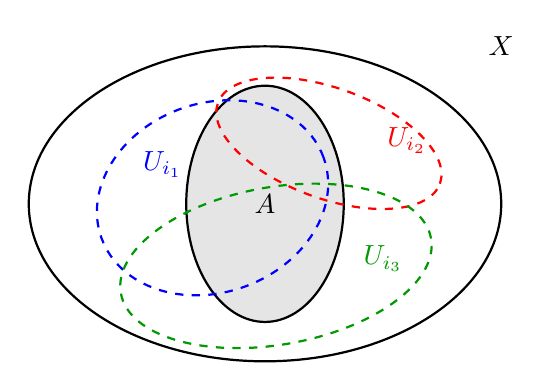
\begin{tikzpicture}
    % Draw the large space X
    \draw[thick] (0,0) ellipse (3 and 2);
    \node at (3, 2) {$X$};

    % Draw the compact subspace A
    \draw[thick, fill=gray!20] (0,0) ellipse (1 and 1.5);
    \node at (0, 0) {$A$};

    % Draw open sets U_i that cover A
    \draw[blue, thick, dashed, rotate=20] (-0.6,0.3) ellipse (1.5 and 1.2);
    \node[blue] at (-1.3,0.5) {$U_{i_1}$};

    \draw[red, thick, dashed, rotate=-20] (0.5,1) ellipse (1.5 and 0.7);
    \node[red] at (1.8, 0.8) {$U_{i_2}$};

    \draw[green!60!black, thick, dashed, rotate=10] (0,-0.8) ellipse (2 and 1);
    \node[green!60!black] at (1.5,-0.7) {$U_{i_3}$};
  \end{tikzpicture}
\end{center}

\begin{proof}
    We show both directions.
    \begin{enumerate}
      \item[\( \Rightarrow \))]
        Assume \( A \) is compact as
        a subspace.
        Let \( \{ U_i \} _{i \in I}\) be a familiy
        of opens in \( X \) such that
        \( A \subseteq \bigcup_{i \in I} U_i \).
        Then \( \bigcup_{i \in I} U_i \cap A \)
        covers \( A \) since
        \[
          \bigcup_{i \in I} U_i \cap A = A \cap \bigcup_{i \in I} U_i = A
        \]
        Now, since \( A \) is compact as a subspace,
        there exists a finite refinement \( J \subseteq I \)
        such that
        \[
          A = \bigcup_{j \in J} U_j \cap A
          \subseteq \bigcup_{j \in J} U_j
        \]
      \item[\( \Leftarrow \))]
        Assume that every family \( \{ U_i \} _{i \in I} \)
        such that \( A \subseteq \bigcup_{i \in I} U_i \)
        admits a finite refinement \( J \subseteq I \) such that
        \[
          A \subseteq \bigcup_{j \in J} U_j
        \]
        Then we need to show that \( A \) is compact as 
        a subspace.
        Pick a cover of \( A \):
        \[
          \{ V_i \}_{i \in I} = \{ U_i \cap A \}_{i \in I}
        \]
        Since \( A \subseteq \bigcup_{i \in I} U_i \),
        then by  assumtion we can refine it and get
        \[
          A = \bigcup_{\alpha = 0}^n V_{i_\alpha}
        \]
    \end{enumerate}
\end{proof}

\begin{theorem}
  \label{thm:compace_sub_closed}
    Let \( X \) be a compact space.
    Let \( A \subseteq X \) be closed.
    Then \( A \) is compact.
\end{theorem}

\begin{proof}
  Let \( \{ U_i \}_{i \in I}  \) be a family of opens such that
   \( A \subseteq \bigcup_{i \in I} U_i \).
    Now since \( A \) closed, then \( A^\mathsf{c} \)
    open. We have that
    \[
      \bigcup_{i \in I} U_i \cup A^\mathsf{c} = X
    \]
    and since \( X \) compact, we have a finite refinement
    \( J \subseteq I \cup *  \).
    Now, \( J \) contains finitely many indices such that
    \( A \subseteq \bigcup_{j \in J} U_j \)
    and by lemma \ref{lma:subspace_compact}, \( A \) is compact.
\end{proof}

\begin{theorem}
  \label{thm:compact->closed}
    Let \( X \) be Hausdorff.
    Given \( K \subseteq X \), \( K \) compact.
    Then \( K \) is closed.
\end{theorem}

\begin{proof}
    Since \( X \) is Hausdorff, we can do the following.
    Let \( x \notin K \).
    For every \(y \in K \),
    pick nbhs. \( U_y \ni x, V_y \ni y \)
    such that \( U_y \cap V_y = \emptyset \).
    Now \( \{ V_y \}_{y \in Y} \) is a cover of \( K \).
    Since
    \( K \) is compact, there exists a finite refinement
    \( J \) such that
    \[
      K \subseteq \bigcup_{j \in J} V_{y_j}
    \]
    Now, let \( U = \cap_{j\in J} U_{y_j} \).
    Note that \( x \in U \) and \( U \) is open.
    Also
    \[
      U \cap K \subseteq U \cap \left(\bigcup_{j \in J} V_{y_j}\right) = \bigcup_{j \in J} U \cap V_{y_j} = \emptyset
    \]
    Since \( x \notin K \) was arbitrary
    \( K^\mathsf{c} \) is open, hence \( K \) is closed.
\end{proof}

Motivation: this theorem makes life easier when we want to prove that
a surjective map is a quotient map by 
combining \ref{thm:compact->closed} and \ref{thm:cont_surj_closed->quotient}.
Here is an example:

\begin{example}
  We want to show that
  \begin{align*}
    f: [0, 1] &\longrightarrow \mathbb{S}^1 \\ t &\longmapsto (\cos 2 \pi t, \sin 2 \pi t)
  \end{align*}
  is a quotient map. 
\end{example}

\begin{proof}
  \( f \) is continuous and surjective.
  Let \( K \subseteq [0, 1] \) closed.
  Since \( [0, 1] \) compact and \( K \) is closed,
 \( K \) is compact by theorem \ref{thm:compace_sub_closed}.
  Now, \( f(K) \subseteq \mathbb{S}^1 \) and since
  \( \mathbb{S}^1 \) is Hausdorff we get that
  \( f(K) \) is closed by theorem \ref{thm:compact->closed}.
  Hence \( f \) is a continuous, surjective and closed map,
  so \( f \) is a quotient map by \ref{thm:cont_surj_closed->quotient}.
\end{proof}


\section{Compact spaces, product of compact spaces is compact.}

\begin{proposition}
    Let \( f: X \to Y \) be a continuous surjection.
    If \( X \) is compact, then \( Y \) is compact.
\end{proposition}

\begin{proof}
  Let \( \{ U_i \}_{i \in I}  \) be a cover of \( Y \).
  Then \( \{ {f}^{-1} (U_i) \}_{i \ in I} \) is a cover of
  \( X \) since \( f \) is continuous.
  Now, \( X \) is compact, so there exists a finite refinement
  of \( I \), say \( J \subseteq I \).
  Now \( \bigcup_{j \in J} U_j = Y \)  since
  \[
    Y = f(X) = f\left(\bigcup_{j \in J} {f}^{-1}(U_j)\right)
    = \bigcup_{j \in J} f\left({f}^{-1}(U_j)\right)
    = \bigcup_{j \in J} U_j
  \]
\end{proof}

\subsection{Product of compact spaces}

\begin{lemma}[Tubular neighborhood lemma]
   Let \( X, Y \) be topological spaces and let \( Y \) be compact.
   Fix \( x \in X \) such that \( U \subseteq X \times Y \) is a open subset of \( X \times Y \)
   and such that \( \{ x  \} \times Y \subseteq U  \).
   Then there exists an open subset \( W_x \subseteq X \) such that \( x \in W_x \) and \( W_x \times Y \subseteq U \).
\end{lemma}

\begin{proof}
  Since \( U \) is open, for all points \( (x, y) \),
  where \( x \) is the fiexd point from the statement,
  we have an open \( W_y \times V_y \subseteq U \).
  Then \( \{ V_y \} _{y \in Y} \) is a cover of 
  \( Y \). But \( Y \) is compact, so there exists
  a finite number of points \( y_0, \dots, y_n \) such that
  \[
  Y = \bigcup_{i \in I} V_{y_i}
  \]
  Let \( W_x = \bigcap_{i \in I} W_{y_i} \).
  \( W_x \) is open since \( I \) is finite.
  Now
  \[
    W_x \times Y \subseteq \bigcup_{i \in I} W_x \times V_{y_i} \subseteq U
  \]
\end{proof}

\begin{theorem}
  Let \( X, Y \) be compact topological spaces.
  Then \( X \times Y \) is compact.
\end{theorem}

\begin{proof}
  Let \( \{ U_i \}_{i \in I}  \) be a cover of
  \( X \times Y \).
  Pick \( x \in X \). Now \( \{ x \} \times Y \simeq Y \),
  and since \( Y \) compact and \( \{ U_i \}_{i \in I}  \)
  covers \( \{ x \} \times Y \)
  we have a finite refinement \( I_x \subseteq I \)
  such that \(\{ x \} \times Y \subseteq  \bigcup_{i \in I_x} U_i \).
  Define \( U_x = \bigcup_{i \in I_x} U_i \).

  By the Tubular neighborhood lemma there exists
  an open subset \( W_x \subseteq U_x \) such that
  \( x \in W_x \) and \( W_x \times Y \subseteq U_x \).

  \( x \) was arbitrary, so we get a cover of \( X \):
  \( \{ W_x \}_{x \in X}  \). \( X \) is compact
  so we pick a finite refinement \( j = 0, \dots, n \) such that
  \( \bigcup_{j = 0}^n W_{x_j} = X \).

  Then
  \[
    \bigcup_{j = 0}^n \bigcup_{i \in I_{x_j}} U_i
    = \bigcup_{j = 0}^n U_{x_j}
    \supseteq \bigcup_{j=0}^n W_{x_j} \times Y = X \times Y
  \] 
  And the double union on the left hand side
  of the equation is finite since it is a
  finite union of a finite union.
\end{proof}

\subsection{The closed interval is compact}

\begin{theorem}
  Let \( [a, b] \) ba a closed interval in \( \mathbb{R} \).
  Then \( [a, b] \) is compact.
\end{theorem}

\begin{proof}
    todo.
\end{proof}

\begin{definition}[boundedness]
    Let \( (X, d) \) be a metric space.
    Then \( A \subseteq X \) is bounded if there exists
    a constant \( L > 0 \) such that \( d(x, y) < L \)  for all \( x, y \in A \).
\end{definition}

\begin{theorem}[Heine-Borel]
  Let \( A \subseteq \mathbb{R}^n \) be a subspace of \( \mathbb{R}^n \).
  Then \( A \) is compact iff. \( A \) is closed and bounded.
\end{theorem}

\begin{proof}
    todo.
    idea: \( \Leftarrow \) by building a square around \( A \). square is product of closed intervals, which are compact.
\end{proof}

\begin{theorem}[Generalised extreme value theorem]
    Let \( f: X \to \mathbb{R} \) be a continuous map.
    If \( X \) is compact then there exist \( m, M \in X \)
    such that \( f(m) \le f(x) \le f(M) \) for all \( x \in X \).
\end{theorem}

\begin{proof}
   todo. 
\end{proof}

Now we can argue that \( f: [0, 1] \to S^1, t \mapsto (\cos 2\pi t, \sin 2\pi t) \) is a quotient map:

\begin{example}
  Let \( Z \subseteq [0, 1]  \) be a closed subset of \( [0, 1] \).
  Since \( [0, 1] \) is compact, \( Z \) is also compact.
  Now \( f \) is a continuous surjection so \( f(Z) \) is compact.
  \( S^1 \) is Hausdorff, so \( f(Z) \) has to be closed.
  Thus \( f \) is closed and \( f \) is thus a quotient map.
\end{example}


\section{Solutions to Exercise sheet 2}
21.02

\section{Homotopy between maps, homotopy as equivalence relation and path homotopy}

\begin{example}
    \( \mathbb{S}^1 \) is compact, but \( \mathbb{R} \) is not.
    So \( \mathbb{S}^1 \not\simeq \mathbb{R} \).
\end{example}

\begin{example}
    \( \mathbb{R} \setminus \{ p \}  \) is not connected.
    Assume that there exists a homeomorphism
    \[
      f: \mathbb{R} \to \mathbb{R}^2
    \]
    \( f \) induces a map
    \[
      \hat{f}: \mathbb{R} \setminus \{ p \}  \to \mathbb{R}^2 \setminus \{ f(p) \} 
    \]
    but \( \mathbb{R}^2 \setminus \{ f(p) \}  \) is connected.
    Hence \( \mathbb{R} \not\simeq \mathbb{R}^2 \).
\end{example}

Denote by \( I \) the closed interval \( [0, 1] \subseteq \mathbb{R} \)
with the usual topology.

\subsection{Homotopy theory}

\subsection{Homotopies}

\begin{definition}[Homotopy]
    Let \( f,g: X \to Y \) be continuous maps
    of topological spaces.
    We say that \( f \) is homotopic to \( g \)
    if there exists a continuous map
    \( H: I \times X \to Y \) such that
    \begin{align}
      H(0, x) &= f(x) \\
      H(1, x) &= g(x)
    \end{align}
    We denote that two maps \( f \) and \( g \) are homotopic
    by writing \( f \simeq g \).
\end{definition}

\begin{definition}[Nullhomotopy]
   A continuous map \( f: X \to Y \)
   is nullhomotopic if it is homotopic
   to a constant map.
\end{definition}

\begin{example}
    Consider two maps \( f, g: X \to \mathbb{R}^n \).
    They are homopotic via the homotopy
    \begin{equation}
        H(t, x) = (1-t) f(x) + t g(x)
    \end{equation}
    Now, \( H \) is continuous, and Fernando says:
    \begin{displayquote}
      If this is not continuous, life has no purpose.
    \end{displayquote}
    To see that \( H \) is continous, consider the following
    diagrams and argue by composition of known continous maps:
    % https://q.uiver.app/#q=WzAsNixbMCwwLCJJIFxcdGltZXMgWCJdLFsyLDAsIlxcbWF0aGJie1J9Xm4gXFx0aW1lcyBcXG1hdGhiYntSfV5uIl0sWzQsMCwiXFxtYXRoYmJ7Un1ebiJdLFswLDEsIih0LHgpIl0sWzIsMSwiKCgxLXQpZih4KSx0Zyh4KSkiXSxbNCwxLCIoMS10KWYoeCkgKyB0Zyh4KSJdLFswLDEsIlxcZ2FtbWFcXHRpbWVzXFx2YXJwaGkiXSxbMSwyLCJcXG9wbHVzIl0sWzMsNF0sWzQsNV1d
\[\begin{tikzcd}
	{I \times X} && {\mathbb{R}^n \times \mathbb{R}^n} && {\mathbb{R}^n} \\
	{(t,x)} && {((1-t)f(x),tg(x))} && {(1-t)f(x) + tg(x)}
	\arrow["{\gamma\times\varphi}", from=1-1, to=1-3]
	\arrow["\oplus", from=1-3, to=1-5]
	\arrow[from=2-1, to=2-3]
	\arrow[from=2-3, to=2-5]
\end{tikzcd}\]
where \( \gamma \) and \( \varphi \) are defined by
% https://q.uiver.app/#q=WzAsNyxbMSwwLCJJIFxcdGltZXMgWCJdLFszLDAsIlxcbWF0aGJie1J9IFxcdGltZXMgXFxtYXRoYmJ7Un1ebiJdLFs1LDAsIlxcbWF0aGJie1J9Xm4iXSxbMSwxLCIodCx4KSJdLFszLDEsIih0LGcoeCkpIl0sWzUsMSwidGcoeCkiXSxbMCwwLCJcXHZhcnBoaToiXSxbMCwxLCJcXHRleHR7aWR9XFx0aW1lcyBnIl0sWzEsMl0sWzMsNF0sWzQsNV1d
\[\begin{tikzcd}
	{\varphi:} & {I \times X} && {\mathbb{R} \times \mathbb{R}^n} && {\mathbb{R}^n} \\
	& {(t,x)} && {(t,g(x))} && {tg(x)}
	\arrow["{\text{id}\times g}", from=1-2, to=1-4]
	\arrow[from=1-4, to=1-6]
	\arrow[from=2-2, to=2-4]
	\arrow[from=2-4, to=2-6]
\end{tikzcd}\]
% https://q.uiver.app/#q=WzAsNyxbMSwwLCJJIFxcdGltZXMgWCJdLFszLDAsIlxcbWF0aGJie1J9IFxcdGltZXMgXFxtYXRoYmJ7Un1ebiJdLFs1LDAsIlxcbWF0aGJie1J9Xm4iXSxbMSwxLCIodCx4KSJdLFszLDEsIih0LGYoeCkpIl0sWzUsMSwiKDEtdClmKHgpIl0sWzAsMCwiXFxnYW1tYToiXSxbMCwxLCJcXHRleHR7aWR9XFx0aW1lcyBmIl0sWzEsMl0sWzMsNF0sWzQsNV1d
\[\begin{tikzcd}
	{\gamma:} & {I \times X} && {\mathbb{R} \times \mathbb{R}^n} && {\mathbb{R}^n} \\
	& {(t,x)} && {(t,f(x))} && {(1-t)f(x)}
	\arrow["{\text{id}\times f}", from=1-2, to=1-4]
	\arrow[from=1-4, to=1-6]
	\arrow[from=2-2, to=2-4]
	\arrow[from=2-4, to=2-6]
\end{tikzcd}\]
From this we conclude that any
two maps with target in \( \mathbb{R}^n \)
are homotopic. In particular, every
map is nullhomotopic.
\end{example}

\begin{definition}
    Let \( X, Y \) be topological spaces.
    Define
    \begin{equation}
      \hom_{\text{Top}}(X, Y) = \{ f:X \to Y \mid f \text{cont.} \} 
    \end{equation}
\end{definition}

\begin{lemma}[Pasting lemma]
   Let \( X = A \cup B \) be a topological space
   where \( A, B \) are closed subsets.
   Suppose  \( f: A \to Y \) and \( g: B \to Y \) are
   continuous maps such that
  \[
    f|_{A\cap B} = g|_{A\cap B}.
  \] 
  Then there exists a continuous map \( h:X \to Y \)
  such that
  \[
    h|_A = f, h|_B = g.
  \]
\end{lemma}

\begin{proof}
    Define \( h:X \to Y \) by
    \[
      h(x) = \begin{cases}
        f(x) & x \in A \\
        g(x) & x \in B
      \end{cases}
    \]
    \( h \) is well defined since \( f \) and \( g \) agree
    on the intersection of \( A \) and \( B \).
    Take a closed subset \( Z \subseteq Y \).
    Then
    \begin{align*}
      {h}^{-1} (Z) &=( {h}^{-1} (Z) \cap A ) \cup ( {h}^{-1} (Z) \cap B ) \\
                   &= {f}^{-1} (Z) \cup {g}^{-1} (Z)
    \end{align*}
    And since \( f, g \) are cont. and \( Z \) closed
    we get that \( {f}^{-1} (Z) \subseteq A \subseteq X \)
    and \( {g}^{-1} (Z) \subseteq B \subseteq X \) are closed.
    Furthermore, a finite union of closed subsets is closed,
    so \( {h}^{-1} (Z) \) is closed.
\end{proof}

\begin{theorem}
   Homotopies are an equivalence relation on  \( \hom_{\text{Top}}(X, Y) \) .
\end{theorem}

\begin{proof} We prove reflexivity, symmetry and transitivity.
    \begin{enumerate}
      \item[1)] Define \( H: I \times X \to X \) by sending
        \( (t, x) \) to \( f(x) \).
        Then \( H(0, x) = H(1,x) = f(x) \).
      \item[2)] Let \( H \) be a homotopy of \( f \) and \( g \).
        Define \( \overline{H} \) by
% https://q.uiver.app/#q=WzAsNixbMSwwLCJJIFxcdGltZXMgWCJdLFszLDAsIkkgXFx0aW1lcyBYIl0sWzUsMCwiWSJdLFsxLDEsIih0LCB4KSJdLFszLDEsIigxLXQsIHgpIl0sWzAsMCwiXFxvdmVybGluZXtIfToiXSxbMCwxXSxbMSwyLCJIIl0sWzMsNF1d
\[\begin{tikzcd}
	{\overline{H}:} & {I \times X} && {I \times X} && Y \\
	& {(t, x)} && {(1-t, x)}
	\arrow[from=1-2, to=1-4]
	\arrow["H", from=1-4, to=1-6]
	\arrow[from=2-2, to=2-4]
\end{tikzcd}\]
Then it is easy to see that \( g \simeq f \).
      \item[3)] Let \( H_1 \) and \( H_2 \) be homotopies
        for \( f \simeq g \) and \( g \simeq h \) respectivly.
        Define
        \begin{equation}
            H_3(t, x) = \begin{cases}
              H_1(2t, x) & 0 \le t \le 1/2 \\
              H_2(2t-1, x) & 1/2 \le t \le 1
            \end{cases}
        \end{equation}
        \( H_3 \) is continuous by the pasting lemma.
        It is easy to check that it is a homotopy.
    \end{enumerate}
\end{proof}

\begin{definition}
    Notation:
    \begin{align}
      [X, Y] &= \hom_{\text{Top}} ( X, Y) / \simeq \\
      [f] &= \{ g: X \to Y \mid f \simeq g, g \in \hom_{\text{Top}} ( X, Y) \}
    \end{align}
\end{definition}

\begin{definition}
    Denote by \( * \) the singelton set.
    \begin{equation}
      [*, Y] = Y / (y_0 \sim y_1 \text{if a path exists}) = \pi_0(Y)
    \end{equation}
\end{definition}

\( Y \) path connected \( \iff \) \( \pi_0(Y) = * \).

\subsection{Path homotopies}

\begin{definition}[Path homotopy]
   Let \( f,g: I \to X \) be paths from
   \( x_0 \) to \( x_1 \).
    We say that \( f \) is path homotopic
    to \( g \) and write \( f \simeq_{p} g \) if
    there exists a continuous function
    \( H: I \times I \to X \) such that
    \begin{align*}
      H(0, s) = f(s)&, H(1, s) = g(s) \\
      H(t, 0) = x_0&, H(t, 1) = x_1
    \end{align*}
\end{definition}

\begin{example}
    Let \( D^2 = \{ (x, y) \in \mathbb{R}^2 \} \mid x^2 + y^2 \le 1  \)
    be the unit disk. Consider \( D^2 \setminus \{ (0, 0) \}  \).
    Then \( f \not\simeq_p g \).
    \begin{center}
      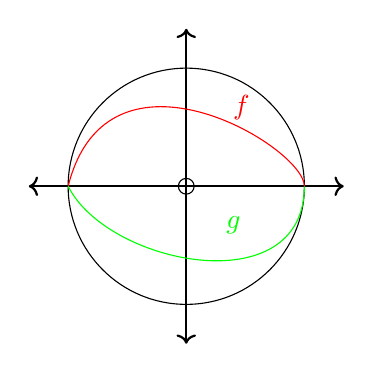
\begin{tikzpicture}
        \draw[thick, <->] (-2, 0)  -- (2, 0);
        \draw[thick, <->] (0, -2)  -- (0, 2);

        \draw (0, 0) circle (1.5);
        \draw (0, 0) circle (0.1);

        \draw[red] (-1.5, 0) .. controls (-1, 2) and (1.5, 0.5) .. (1.5, 0) node at (0.7,1) {\( f \)};
        \draw[green] (-1.5, 0) .. controls (-1, -1) and (1.5, -1.5) .. (1.5, 0) node at (0.6, -0.5) {\( g \)};
      \end{tikzpicture}
    \end{center}
\end{example}

\begin{definition}
  \( \hom_{\text{Top}}^{x_0, x_1} = \{ f: I \to X \mid f \text{cont.}, f(0) = x_0, f(1) = x_1  \}  \).
\end{definition}

\begin{theorem}
    Path homotopies define an equivalence relation on \( \hom_{\text{Top}}^{x_0, x_1} \).
\end{theorem}

\begin{proof}
    Similar as the proof of homotopy equivalence relation.
\end{proof}

\section{Concatenation of paths, associativity , unitality}
20.02

\begin{definition}
    Fernando notation:
    \[
      X(x_0, x_1) = \hom_{\text{Top}}^{x_0,x_1}(I, X) / \simeq_p
    \]
\end{definition}


\begin{example}
    \( \mathbb{R}^n(x_0, x_1) = * \).
\end{example}

\begin{definition}[loop]
    A loop is a path from \( x \) to \( x \).
\end{definition}

\begin{definition}[path concatination]
   Let \( f, g: I \to X \) be paths from
   \( x_0  \) to \( x_1 \) and from \( x_1 \)
   to \( x_2 \) respectivly.
   Define the concatination of \( f \) and \( g \) as:
  \begin{equation}
      (g * f)(s) = \begin{cases}
          f(2s) & 0 \le s \le 1/2 \\
          g(2s - 1) & 1/2 \le s \le 1
      \end{cases}
  \end{equation}
\end{definition}

\begin{proposition}
    Path concatination is a well defined operation
    on path homotopy equivalence classes. That is:
    \begin{align*}
      X(x_0,x_1) \times X(x_1, x_2) &\longrightarrow X(x_0, x_2) \\
      ([f], [g]) &\longmapsto [g * f]
    \end{align*}
    is well defined.
\end{proposition}

\begin{proof}
  Let \( f, f': I \to X \) be path homotopic maps
    from \( x_0 \) to \( x_1 \).
  Let \( g, g': I \to X \) be path homotopic maps
    from \( x_1 \) to \( x_2 \).
  Hence, \( f, f' \in [f] \) and \( g, g' \in [g] \).
  We need to show that
    \[
      g * f \simeq_p g' * f'.
    \]
  Let \( H_1 \) be a path homotopy of \( f \) and \( f' \).
  Let \( H_2 \) be a path homotopy of \( g \) and \( g' \).
  Define
  \[
    H_3(t, s) = \begin{cases}
      H_1(t, 2s) & 0 \le s \le 1/2 \\
      H_2(t, 2s -1) & 1/2 \le s \le 1
    \end{cases}
  \]
  \( H_3 \) is well defined since
  \[
    H_3(t, 1/2) = \begin{cases}
      H_1(t, 1) \\
      H_2(t, 0) 
    \end{cases}
    = \begin{cases}
        x_1 \\ x_1
    \end{cases}
    = x_1
  \]
  Check that \( H_3 \) is a path homotopy of 
  \( g * f \) and \( g' * f' \).
  \begin{enumerate}
    \item 
      \begin{align*}
        H_3(0, s) &= \begin{cases}
          H_1(0, 2s) & 0 \le s \le 1/2 \\
          H_2(0, 2s -1) & 1/2 \le s \le 1
          \end{cases} \\
                  &= \begin{cases}
          f(2s) & 0 \le s \le 1/2 \\
          g(2s - 1) & 1/2 \le s \le 1
        \end{cases} \\
                  &= (g * f) (s)
      \end{align*}

    \item 
      \begin{align*}
        H_3(1, s) &= \begin{cases}
          H_1(1, 2s) & 0 \le s \le 1/2 \\
          H_2(1, 2s -1) & 1/2 \le s \le 1
          \end{cases} \\
                  &= \begin{cases}
          f'(2s) & 0 \le s \le 1/2 \\
          g'(2s - 1) & 1/2 \le s \le 1
        \end{cases} \\
                  &= (g' * f') (s)
      \end{align*}
  \end{enumerate}
\end{proof}

Notation: Only \( f \) might be used 
instead of \( [f] \) for the equivalence class.

\begin{theorem}
    The operation of concatination
    enjoys the following properties:
    \begin{enumerate}
      \item[1)] Associativity.
        \[
          (h * g) * f \simeq_p h * (g * f)
        \]
      \item[2)] Left/right units.
        \[
          f * c_x \simeq_p f \simeq_p c_y * f
        \]
      \item[3)] Left/right inverses.
        \[
          f * \overline{f} \simeq_p c_y, \overline{f} * f  \simeq_p c_x
        \]
    \end{enumerate}
\end{theorem}

\begin{proof}
  We show the three properties.
  \begin{enumerate}
    \item Associativity.
      Let \( f \in X(x_0, x_1), g \in X(x_1, x_2), h \in X(x_2, x_3) \).
      We have the following
      \begin{align}
        \left(\left(h * g\right) * f\right)(s) &= \begin{cases}
          f(2s) & 0 \le s \le 1/2 \\
          g(4s - 2) & 1/2 \le s \le 3/4 \\
          h(4s - 3) & 3/4 \le s \le 1 \\
                    \end{cases} \\
          \left(h * \left(g * f\right)\right)(s) &= \begin{cases}
          f(4s) & 0 \le s \le 1/4 \\
          g(4s - 1) & 1/4 \le s \le 1/2 \\
          h(2s - 1) & 1/2 \le s \le 1 \\
        \end{cases}
      \end{align}
      A path homotopy for \( (h * g) * f \) and \( h * (g * f) \) is
      \begin{equation}
          H(t, s) = \begin{cases}
            f\left(\frac{4s}{1+t}\right) & 0 \le s \le \frac{1+t}{4} \\
            g\left(4s - t - 1\right) & \frac{1+t}{4} \le s \le \frac{2+t}{4} \\
            h\left(\frac{4s-t-2}{2-t}\right) & \frac{2+t}{4} \le s \le 1
          \end{cases}
      \end{equation}
      \( H \) is continuous by the pasting lemma. And
      \begin{align}
        H(0, s)  &= \begin{cases}
          f(4s) & 0 \le s \le 1/4 \\
          g(4s - 1) & 1/4 \le s \le 1/2 \\
          h(2s - 1) & 1/2 \le s \le 1
        \end{cases} 
                 &= \left(h * \left(g * f\right)\right)(s) \\
          H(1, s) &= \begin{cases}
            f(2s) & 0 \le s \le 1/2 \\
            g(4s - 2) & 1/2 \le s \le 3/4 \\
            h(4s - 3) & 3/4 \le s \le 1
            \end{cases} 
                  &= \left((h * g) * f\right)(s) \\
            H(t, 0) &= f(0) = x_0 \\
            H(t, 1) &= h(1) = x_3
      \end{align}
      Which shows that \( H \) is indeed a path homotopy.

    \item Left/right units.
      Let \( c_x \) be the constant path at \( x \) and
      let \( f \) be a path from \( x \) to \( y \).
      We show that \( f * c_x \simeq_p f \).
      \begin{align}
        (f * c_x)(s) &= \begin{cases}
          x & 0 \le s \le 1/2 \\
          f(2s - 1) & 1/2 \le s \le 1
        \end{cases}
      \end{align}
      The following homotopy works.
      \begin{align}
        H(t, s) &= \begin{cases}
          x & 0 \le s \le \frac{1 - t}{2} \\
          f(2s - 1) & 1/2 \le s \le 1
        \end{cases}
      \end{align}
      It is continuous by the pasting lemma once again.
      We check:
      \begin{align}
        H(0, s) &= \begin{cases}
          x & 0 \le s \le 1/2 \\
          f(2s - 1) & 1/2 \le s \le 1
        \end{cases}
                &= \left(f * c_x\right)(s) \\
          H(1, s) &= \begin{cases}
            x & 0 \le s \le 0 \\
            f(s) & 0 \le s \le 1
          \end{cases}
                  &= f(s) \\
            H(t, 0) &= x\\
            H(t, 1) &= y
      \end{align}
      Hence, \( f * c_x \simeq_p f \).
      Showing that \( c_y \simeq_p f \) follows the same argument.
    \item Left/right inverses.
      Let \( f \) be a path from \( x_0  \) to \( x_1 \).
      Let \( \overline{f} \) be defined by
      \( \overline{f}(t) = f(1-t) \).
      We show that \( \overline{f} * f \simeq_p c_{x_0} \).
      \begin{align}
          (\overline{f} * f)(s) &= \begin{cases}
            f(2s) & 0 \le s \le 1/2 \\
            f(2 - 2s) & 1/2 \le s \le 1
        \end{cases}
      \end{align}
      Define
      \begin{align}
        H(t, s) &= \begin{cases}
          x_0 & 0 \le s \le t/2 \\
          f(2s - t) & t/2 \le s \le 1/2 \\
          f(2 - 2s - t) & 1/2 \le s \le 1 - t/2 \\
          x_0 & 1 - t/2 \le s \le 1
        \end{cases}
      \end{align}
      Then
      \begin{align}
        H(0, s) &= \begin{cases}
          f(2s) & 0 \le s \le 1/2 \\
          f(2 - 2s) & 1/2 \le s \le 1
        \end{cases} &= (\overline{f} * f)(s) \\
        H(1, s) &= \begin{cases}
          x_0 & 0 \le s \le 1/2 \\
          f(2s - 1) & 1/2 \le s \le 1/2 \\
          f(2 - 2s - 1) & 1/2 \le s \le 1/2 \\
          x_0 & 1/2 \le s \le 1
        \end{cases} &= c_{x_0}(s) \\
        H(t, 0) &= x_0 \\
        H(t, 1) &= x_0
      \end{align}
  \end{enumerate}
  Again, showing \( c_{x_1} \simeq_p f * \overline{f} \)
  is similar.
\end{proof}

Fernando defines a group and group homomorphisms.
See wikipedia article on groups.

\begin{definition}[Fundamental group]
   Let \( X \) be a topological space and
   let \( x_0 \in X \) be a point.
   Define the fundamental group of \( X \) at \( x_0 \)
   as
   \begin{align*}
     \pi_1(X, x_0) &= X(x_0, x_0) \\
                   &= \{ f: I \to X \mid f(0) = f(1) = x_0 \} / \simeq_p
   \end{align*}
\end{definition}

\[
  \text{Top} \xrightarrow{\sim} \text{Grp}
\]

\begin{theorem}
    Let \( X \) be a topological space.
    Let \( \alpha: I \to X \) be a path
    from \( x_0 \) to \( x_1 \).
    Then there exists a group isomorphism
    \[
      T_\alpha: \pi_1(X, x_0) \to \pi_1(X, x_1)
    \]
\end{theorem}

\begin{center}
  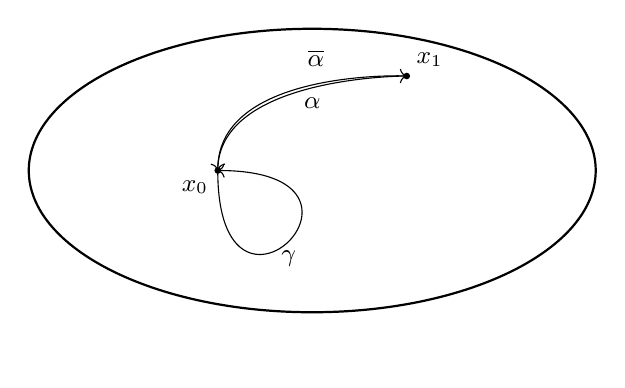
\begin{tikzpicture}[scale=1.2, every node/.style={font=\small}]
    % Draw the boundary of the space
    \draw[thick] (0,0) ellipse (3 and 1.5);

    % Points x0 and x1
    \fill (-1,0) circle (1pt) node[below left] {$x_0$};
    \fill (1,1) circle (1pt) node[above right] {$x_1$};

    % Path from x0 to x1
    \draw[->] (-1,0) .. controls (-1, 1) and (1, 1) .. (1, 1)
      node[midway, below] {$\alpha$};

    % Path from x1 to x0 (reversed)
    \draw[->] (1, 1) .. controls (1.1, 1) and (-1, 1.1) .. (-1, 0)
      node[midway, above=3pt] {$\overline{\alpha}$};

    % Loop \gamma at x0
    \draw[->] (-1, 0) .. controls (-1,-2) and (1,0) .. (-1, 0)
      node[midway, below] {$\gamma$};
  \end{tikzpicture}
\end{center}

\begin{proof}
  Define \( T_\alpha (\gamma) = \alpha * \gamma * \overline{\alpha} \).
  We show that \( T_\alpha \) is an isomorphism of groups.
  First,
  \begin{align*}
    T_\alpha(\varphi * \gamma) &= \alpha * \varphi * \gamma * \overline{\alpha} \\
                               &= \alpha * \varphi * \overline{\alpha} * \alpha * \gamma * \overline{\alpha} \\
                               &= T_\alpha(\varphi) * T_\alpha(\gamma)
  \end{align*}
  so \( T_\alpha \) is a group homomorphism.
  \( T_\alpha \) is bijective, since \( T_{\overline{\alpha}} \)
  is the inverse:
  \begin{align*}
    (T_{\overline{\alpha}} \circ T_{\alpha}) (\gamma)
      &= \overline{\alpha} * \alpha * \gamma * \overline{\alpha} * \alpha = \gamma \\
      (T_{\alpha} \circ T_{\overline{\alpha}}) (\gamma)
      &= \alpha * \overline{\alpha} * \gamma * \alpha * \overline{\alpha} = \gamma
  \end{align*}
\end{proof}

\section{Fundamental group, fundamental group of a product of spaces}
06.03

\begin{definition}[Simply connected]
    A topological space \( X \) is simply connected
    if it is path connected and \( \pi_1(X, x_0) \)
    is trivial.
\end{definition}

\begin{example}
   \( \mathbb{R}^n \) is simply connected.
\end{example}

\begin{definition}[Based space]
   A based space is a pair \( (X, x_0) \) 
   where \( X \) is a topological space
   and \( x_0 \in X \) is a point.
\end{definition}

\begin{definition}[Based map]
   A based map \( f: (X, x_0) \to (Y, y_0) \) 
   is a continuous map such that \( f(x_0) = f(y_0) \).
\end{definition}

\begin{proposition}
  \label{prop:based_grp_hom}
  Let \( f: (X, x_0) \to (Y, y_0) \) be a
  based map. Then there exists a group homomorphism
  \[ f_* = \pi_1(f): \pi_1(X, x_0) \to \pi_1(Y, y_0) \]
\end{proposition}

\begin{proof}
    IDEA: define \( f_*(\gamma) = f\circ \gamma \).
    Show well-definedness and show that it is a grp. hom.
    We define \( f_* = \pi_1(f) \) by 
    \[
      f_*(\gamma) = \left(\pi_1(f)\right)(\gamma) = f \circ \gamma
    \]
    This is a well defined map; take \( \gamma \simeq_p \gamma' \).
    Then
    \[
      f \circ H: I \times I \to X \to Y
    \]
    is a homotopy of \( f_*(\gamma) \) and \( f_*(\gamma') \):
    \begin{enumerate}
      \item \( (f \circ H)(0, s) = (f \circ \gamma)(s)) \).
      \item \( (f \circ H)(1, s) = (f \circ \gamma')(s) \).
      \item \( (f \circ H)(t, 0) = f(x_0) = y_0 \).
      \item \( (f \circ H)(t, 1) = f(x_0) = y_0 \).
    \end{enumerate}
    \( f_* \) is a homomorphism of groups.
    Take \( \gamma_1, \gamma_2 \in \pi_1(X, x_0) \).
    Then
    \begin{align*}
      f_*(\gamma_2) * (f_*(\gamma_1))
      &= \begin{cases}
        (f \circ \gamma_1) (2s)     & 0 \le s \le 1/2 \\
        (f \circ \gamma_2) (2s - 1) & 1/2 \le s \le 1
      \end{cases} = f_*(\gamma_2 * \gamma_1)
    \end{align*}
\end{proof}

\subsection{Category theory}

\begin{definition}[Category]
   A category \( \mathcal{C} \) is
   given by the following
   \begin{itemize}
      \item a set of objects \( \text{ob}(\mathcal{C}) \).
       Notation: \( X \in \mathcal{C} \) means \( X \in \text{ob}(\mathcal{C}) \).
      \item for every object pair \( X, Y \in \text{ob}(\mathcal{C}) \)
        a set \( \mathcal{C}(X, Y) \) of morphisms from \( X \) to \( Y \).
      \item for every \( X, Y, Z \in \mathcal{C} \) a map
        \begin{align*}
          \mathcal{C}(X, Y) \times \mathcal{C}(Y, Z) &\to \mathcal{C}(X, Z) \\
          (f, g) &\mapsto g \circ f
        \end{align*}
      \item Composition of morphisms is associative.
      \item For all \( X \in \mathcal{C} \) there exists a morphism
          \( I_x \in \mathcal{C}(X, X) \) called the identity such that
          \[
            I_x \circ f = f, g \circ I_x = g
          \]
          for all \( f: a \to X \), \( g: X \to b \).
   \end{itemize}
\end{definition}

\begin{example}
    Let \textbf{Set} be the category whose objects are sets
    and whose morphisms are functions.
\end{example}

\begin{example}
    Let \textbf{Top} be the category whose objects are topological spaces
    and whose morphisms are continuous functions.
\end{example}

\begin{example}
    Let \textbf{Grp} be the category whose objects are groups
    and whose morphisms are group homomorphisms.
\end{example}

\begin{example}
    Let \( \textbf{Top}_* \) be the category whose objects are based spaces
    and whose morphisms are based maps.
\end{example}

\begin{definition}[isomorphism]
   Let \( \mathcal{C} \) be a category.
   A morphism \( f: X \to Y \) is an isomorphism
   if there exists a morphism \( g: Y \to  X \) such that
   \begin{align*}
     f \circ g &= I_Y \\
     g \circ f &= I_X
   \end{align*}
\end{definition}

\begin{definition}[functor]
   Let \( \mathcal{C}, \mathcal{D} \) be categories.
   A functor
   \[
    F: \mathcal{C} \to \mathcal{D}
   \]
   is given by functions
   \begin{align*}
     \text{ob}(\mathcal{C}) &\longrightarrow \text{ob}(D) \\
      c &\longmapsto F(c) \\
    \end{align*}
    and
    \begin{align*}
      \mathcal{C}(C, Y) &\longrightarrow \mathcal{D}(F(X), F(Y)) \\
      f &\longmapsto F(f)
    \end{align*}
    that satisfy
    \begin{align*}
      F(g \circ f) &= F(g) \circ F(f) \\
      F(I_X) &= I_{F(X)}
    \end{align*}
\end{definition}

\begin{lemma}
  \label{lma:iso}
    Let \( F: \mathcal{C} \to \mathcal{D} \) be a functor.
    Then \( F \) preserves isomorphisms.
\end{lemma}

\begin{proof}
   Let \( f \) be iso.
   Then we have
   \begin{align*}
     F(I_X) &= I_{F(X)} = F(g \circ f) = F(g) \circ F(f) \\
     F(I_Y) &= I_{F(Y)} = F(f \circ g) = F(f) \circ F(g)
   \end{align*}
   so \( F(f) \) iso.
\end{proof}

\begin{example}
    There is a functor
    \[
      \mathbf{Grp} \xrightarrow{U} \mathbf{Set}
    \]
    that is forgetful.
\end{example}

\begin{theorem}
    The fundamental group is a functor
    \[
      \pi_1: \mathbf{Top}_* \longrightarrow \mathbf{Grp}
    \]
\end{theorem}

\begin{proof}
  Given \( (X, x_0), (Y, y_0) \) based spaces
  and \( f, g: (X, x_0) \to (Y, y_0) \) based maps.
  Proposition \ref{prop:based_grp_hom} gives 
  the group homomorphism we need:
  \begin{align*}
    \pi_1(f) = f_* : \pi_1(X, x_0) &\longrightarrow \pi_1(Y, y_0) \\
    [\gamma] &\longmapsto [f \circ \gamma]
  \end{align*} 
  The identity map is sent to the identity map:
% https://q.uiver.app/#q=WzAsNixbMCwwLCIoWCx4XzApIl0sWzIsMCwiKFgseF8wKSJdLFswLDIsIlxccGlfMShYLHhfMCkiXSxbMiwyLCJcXHBpXzEoWCx4XzApIl0sWzAsMywiW1xcZ2FtbWFdIl0sWzIsMywiW1xcdGV4dHtpZH0gXFxjaXJjIFxcZ2FtbWFdIl0sWzAsMSwiXFx0ZXh0e2lkfSJdLFsyLDMsIlxcdGV4dHtpZH0iLDJdLFs0LDUsIiIsMCx7InN0eWxlIjp7InRhaWwiOnsibmFtZSI6Im1hcHMgdG8ifX19XSxbNiw3LCJcXHBpXzEiLDAseyJzaG9ydGVuIjp7InNvdXJjZSI6MjAsInRhcmdldCI6MjB9fV1d
\[\begin{tikzcd}
	{(X,x_0)} && {(X,x_0)} \\
	\\
	{\pi_1(X,x_0)} && {\pi_1(X,x_0)} \\
	{[\gamma]} && {[\text{id} \circ \gamma]}
	\arrow[""{name=0, anchor=center, inner sep=0}, "{\text{id}}", from=1-1, to=1-3]
	\arrow[""{name=1, anchor=center, inner sep=0}, "{\text{id}}"', from=3-1, to=3-3]
	\arrow[maps to, from=4-1, to=4-3]
	\arrow["{\pi_1}", shorten <=9pt, shorten >=9pt, Rightarrow, from=0, to=1]
\end{tikzcd}\]
and preserve compositions. Composing in \( \mathbf{Grp} \):
% https://q.uiver.app/#q=WzAsNixbMCwwLCJcXHBpXzEoWCwgeF8wKSJdLFsyLDAsIlxccGlfMShZLCB5XzApIl0sWzQsMCwiXFxwaV8xKFosIHpfMCkiXSxbMCwxLCJbXFxnYW1tYV0iXSxbMiwxLCJbZiBcXGNpcmMgXFxnYW1tYV0iXSxbNCwxLCJbZyBcXGNpcmMgZiBcXGNpcmMgXFxnYW1tYV0iXSxbMCwxLCJmXyoiXSxbMSwyLCJnXyoiXSxbMyw0LCIiLDAseyJzdHlsZSI6eyJ0YWlsIjp7Im5hbWUiOiJtYXBzIHRvIn19fV0sWzQsNSwiIiwwLHsic3R5bGUiOnsidGFpbCI6eyJuYW1lIjoibWFwcyB0byJ9fX1dXQ==
\[\begin{tikzcd}
	{\pi_1(X, x_0)} && {\pi_1(Y, y_0)} && {\pi_1(Z, z_0)} \\
	{[\gamma]} && {[f \circ \gamma]} && {[g \circ f \circ \gamma]}
	\arrow["{f_*}", from=1-1, to=1-3]
	\arrow["{g_*}", from=1-3, to=1-5]
	\arrow[maps to, from=2-1, to=2-3]
	\arrow[maps to, from=2-3, to=2-5]
\end{tikzcd}\]
First composing in \(\textbf{Top}_*\):
% https://q.uiver.app/#q=WzAsNCxbMCwwLCJcXHBpXzEoWCwgeF8wKSJdLFs0LDAsIlxccGlfMShaLCB6XzApIl0sWzAsMSwiW1xcZ2FtbWFdIl0sWzQsMSwiWyhnIFxcY2lyYyBmKSBcXGNpcmMgXFxnYW1tYV0iXSxbMCwxLCIoZyBcXGNpcmMgZilfKiJdLFsyLDNdXQ==
\[\begin{tikzcd}
	{\pi_1(X, x_0)} &&&& {\pi_1(Z, z_0)} \\
	{[\gamma]} &&&& {[(g \circ f) \circ \gamma]}
	\arrow["{(g \circ f)_*}", from=1-1, to=1-5]
	\arrow[from=2-1, to=2-5]
\end{tikzcd}\]
which are equal since, \( g \circ f \circ \gamma = (g \circ f) \circ \gamma\).
\end{proof}

\begin{corollary}
    Let \( X, Y \) be topological spaces and suppose \( X \simeq Y \).
    Then \( \forall x_0 \in X \) we have that
    \( \pi_1(X, x_0) \simeq \pi_1(Y, f(x_0)) \).
\end{corollary}

\begin{proof}
    Since \( X \simeq Y \), we have a homeomorphism \( f: X \to Y \).
    This induces the map  
    \begin{equation*}
      \left(X, x_0\right) \to \left(Y, f(x_0)\right)
    \end{equation*}
    By lemma \ref{lma:iso} we get an isomorphism of groups
    \( \pi_1(X, x_0) \simeq \pi_1(Y, f(x_0) )\).
\end{proof}

\begin{theorem}
    Let \( (X, x_0), (Y, y_0) \) be based spaces.
    Then there exists a canonical isomorphism of groups
    \begin{equation}
      \pi_1(X \times Y, (x_0, y_0)) \xrightarrow{\sim} \pi_1(X, x_0) \times \pi_1(Y, y_0)
    \end{equation}
\end{theorem}

\begin{proof}
The projection maps
\begin{align*}
  p_X: (X \times Y, (x_0, y_0)) &\to (X, x_0) \\
  p_Y: (X \times Y, (x_0, y_0)) &\to (Y, y_0)
\end{align*}
and their images under \( \pi_1 \) induces a
map
\begin{align*}
   \phi: \pi_1(X \times Y, (x_0, y_0)) \to \pi_1(X, x_0) \times \pi_1(Y, y_0)
\end{align*}
defined by
\begin{align}
  \phi([f]) = ([p_X \circ f], [p_Y \circ f]) = ([f_X], [f_Y])
\end{align}
\( \phi \) is a group homomorphism. Let \( [f], [f'] \in \pi_1(X \times Y, (x_0, y_0)) \).
\begin{align*}
  \phi([f] * [f']) &= ([p_X \circ (f*f')], [p_Y \circ (f*f')]) \\
                   &= ([p_X \circ f] * [p_X \circ f'], [p_Y \circ f] * [p_Y \circ f']) \\
                   &= ([p_X \circ f], [p_Y \circ f]) * ([p_X \circ f'], [p_Y \circ f']) \\
                   &= \phi([f])*\phi([f'])
\end{align*}
Now we need to show that \( \phi \) is a bijection.
First we show injectivity.
Assume that \( \phi([f]) = ([f_X], [f_Y]) = ([c_{x_0}], [c_{y_0}]) \) is the identity.
Let \( H_X, H_Y \) be the two path homotopies.
The universal property of the product gives the map
\begin{align*}
  H: I \times I &\to X \times Y \\
  (t, s) &\mapsto (H_X(t, s), H_Y(t, s))
\end{align*}
which is a path homotopy of \( f \simeq_p c_{(x_0, y_0)} \):
\begin{align*}
  H(t, 0) &= H(t, 1) = (H_X(t, 0), H_Y(t, 0)) = (H_X(t, 1), H_Y(t, 1)) = (x_0, y_0) \\
  H(0, s) &= (H_X(0, s), H_Y(0, s)) = (f_X, f_Y) \\
  H(1, s) &= (H_X(1, s), H_Y(1, s)) = (c_{x_0}, x_{y_0})
\end{align*}
Now we show surjectivity:
Given \( ([\alpha], [\beta]) \in \pi_1(X, x_0) \times \pi_1(Y, y_0) \)
we see that \( \phi([(\alpha, \beta)]) = ([\alpha], [\beta]) \).
\end{proof}

\section{Solutions to Exercise sheet 3}
14.03

Exercises. Maybe add these in the future.


\section{Homotopy equivalences and the fundamental group}
20.03

\begin{definition}
    Let \( f,g: (X, x_0) \to (Y, y_0) \) be based maps
    We say that a homotopy
    \[
      H: I \times X \to Y
    \]
    is a based homotopy if \( H(t, x_0) = y_0 \)
    for all \( t \).
\end{definition}

\begin{lemma}
  \label{lma:based_maps_homotopic}
    Let \( f, g: (X, x_0) \to (Y, y_0) \)
    be based maps which are homotopic via
    a based homotopy. Then
    \[
      \pi_1 (f) = \pi_1(g)
    \]
\end{lemma}

\begin{proof}
    Let \( \gamma \in \pi_1(X, x_0) \).
    We need to show that \( f_*(\gamma) \simeq_p g_*(\gamma) \).
    That is, there exists a path homotopy
    for \( f \circ \gamma \) and \( g \circ \gamma \).
    Let \( H: I \times X \to X \) be a based homotopy
    for \( f \) and \( g \).
    Then
    \[
      \hat{H}: I \times I \xrightarrow{\text{id} \times \gamma}
      I \times X \xrightarrow{H} Y
    \]
    is this path homotopy.
    \begin{enumerate}
      \item \( \hat{H}(0, s) = H(0, \gamma(s)) = (f \circ \gamma) (s) \)
      \item \( \hat{H}(1, s) = H(1, \gamma(s)) = (g \circ \gamma) (s) \)
      \item \( \hat{H}(t, 0) = H(t, \gamma(0)) = y_0 \)
      \item \( \hat{H}(t, 1) = H(t, \gamma(1)) = )y_0 \)
    \end{enumerate}
\end{proof}

\begin{definition}[retract, retraction]
   Let \( A \subseteq X \) be a subspace.
   We say that \( A \) is a retract of \( X \)
   if there exists a map
   \[
    r: X \to A
   \]
   such that \( r \circ \iota = \text{id}_A \).
   We call \( r \) a retraction.
\end{definition}


\begin{example}
   Consider \( \mathbb{S}^1 \subseteq \mathbb{R}^2 \setminus \{ (0, 0) \}  \) .
   Then \( r(x) = x / \lvert \lvert x \rvert \rvert \) is a retraction.
\end{example}

\begin{lemma}
  \label{lma:retract->inj}
  Let \( x_0 \in A \subseteq X  \), and suppose
  that \( A \) is a retract of \( X \).
  Then the induced group homomorphism
  \[
    \pi_1(A, x_0) \longrightarrow \pi_1(X, x_0)
  \]
  is injective.
\end{lemma}

\begin{proof}
   Let \( r: X \to A \) be a retraction.
    Since \( x_0 \in A \) then \( r(x_0) = x_0 \).
    I get group homomorphisms
    \begin{equation}
      \pi_1(A, x_0) \xrightarrow{\pi_1(\iota)} \pi_1(X, x_0)
      \xrightarrow{\pi_1(r)} \pi_1(A, x_0)
    \end{equation}
    That compose to the identity: \( \pi_1(r) \circ \pi_1(\iota) = id \).
    Since the composite is injective, \( \pi_1(\iota) \) is injective.
\end{proof}

\begin{definition}[deformation retract]
    Let \( A \subseteq X \) be a subspace.
    A homotopy
    \[
      H: I \times X \to X
    \]
    is a deformation retract if the following holds
    \begin{enumerate}
      \item \( H(0, x) = x \)
      \item \( H(1, x) \in A \)
      \item \( H(t, a) = a, \forall a \in A \)
    \end{enumerate}
\end{definition}

\begin{remark}
   A deformation retract is a retract. 
\end{remark}

\begin{proof}
    Let \( A \subseteq X \) and \( H: I\times X \to X \)
    be a deformation retract. Then we get the retract
    \( r: X \to A \) by
    \[
      H(1, x): X \xrightarrow{r} A \xrightarrow{\iota} X
    \]

\end{proof}

\begin{theorem}
    Let \( x_0 \in A \subseteq X \) and suppose
    that \( A \) is a deformation retract of \( X \).
    Then we have a group isomorphism
    \[
      \pi_1(\iota): \pi_1(A, x_0) \to \pi_1(X, x_0)
    \]
\end{theorem}

\begin{proof}
  My notes here are hardly intelligible, so I provide
  my own proof. (I think this is what Fernando wrote).

  By lemma \ref{lma:retract->inj}
  \( \pi_1(\iota) \) is an injective group homomorphism.
  We need to show that it is surjective, i.e. that
  \( \pi_1(\iota) \circ \pi_1(r) = \text{id}  \).
  Let \( H: I \times X \to X \) be the
  deformation retract.
  Let \( H(1, x) = r: X \to A \) denote the retract.
  Now, \( H \) is a based homotopy of \( \text{id} \) and
  \( r \circ \iota  \):
  \begin{align*}
    H(t, x_0) &= x_0 & \text{since \( x_0 \in A \). } \\
    H(0, x) &= x \\
    H(1, x) &= \left(\iota \circ r\right)(x)
  \end{align*}
  By lemma \ref{lma:based_maps_homotopic}
  \( \pi_1(\iota) \circ \pi_1(r) = \text{id} \),
  so \( \pi_1(\iota) \) is surjective.

  Hence, \( \pi_1(\iota) \) is an isomorphism
  of groups.
\end{proof}

\begin{exercise}
    Show that \( \mathbb{S}^1 \subseteq \mathbb{R}^2 \setminus \{ (0, 0) \}  \)
    is a deformation retract.
\end{exercise}

\begin{definition}[homotopy equivalence]
    A map \( f: X \to Y \) is a homotopy equivalence
    if there exists a continuous map
    \[
      g: Y \to X
    \]
    such that \( g \circ f \sim \text{id}_X \)
    and \( f \circ g \sim \text{id}_Y \).
\end{definition}

\begin{example}
  Let \( A \subseteq X \) be a deformation retract.
  Then \( \iota: A \to X \) is a homotopy equivalence.
\end{example}

\begin{example}
    \( 0 \in \mathbb{R}^n \). \( \mathbb{R}^n \sim * \).
\end{example}

\begin{definition}[Contractible space]
   A space is said to be contractible
   if it is homotopy equivalent to
   the point space.
\end{definition}

\begin{definition}[homotopy type]
    We say that \( X \) and \( Y \)
    have the same homotopy type if \( X \)
    is homotopy equivalent to \( Y \).
    Notation:
    \[
      [X] = \{ Y \text{top. space} \mid X \text{ homotopic equivalent to } Y \} 
    \]
\end{definition}

\begin{example}
  \( [\mathbb{R}^n] = [*] \).
\end{example}

\begin{lemma}
  \label{lma:hom_diag_lemma}
    Let \( f, g: X \to Y \) be maps.
    Suppose \( H \) is a homotopy
    \[
      H: I \times X \to Y
    \]
    between \( f, g \).
    Given \( x_0 \in X \), and let
    \[
      \alpha = H(\cdot, x_0): I \to X
    \]
    Then we have a commutative diagram 
    of groups:

    % https://q.uiver.app/#q=WzAsMyxbMCwwLCJcXHBpXzEoWCwgeF8wKSJdLFsyLDIsIlxccGlfMShZLCBnKHhfMCkpIl0sWzIsMCwiXFxwaV8xKFksIGYoeF8wKSkiXSxbMCwxLCJcXHBpXzEoZykiLDJdLFswLDIsIlxccGlfMShmKSJdLFsyLDEsIlxcaGF0e1xcYWxwaGF9Il1d
\[\begin{tikzcd}
	{\pi_1(X, x_0)} && {\pi_1(Y, f(x_0))} \\
	\\
	&& {\pi_1(Y, g(x_0))}
	\arrow["{\pi_1(f)}", from=1-1, to=1-3]
	\arrow["{\pi_1(g)}"', from=1-1, to=3-3]
	\arrow["{\hat{\alpha}}", from=1-3, to=3-3]
\end{tikzcd}\]
where \( \hat{\alpha}([\gamma]) = [\alpha * \gamma * \overline{\alpha}] \).
\end{lemma}

\begin{proof}
   We need to show that
   \( \hat{\alpha} \circ \pi_1(f) = \pi_1(g) \).
   That is;
   \[
     [\alpha * (f \circ \gamma) * \overline{\alpha}]
     = [g \circ \gamma]
   \]
   for all \( \gamma \in \pi_1(X, x_0) \).
  Let \( \gamma  \) be a loop based at \( x_0 \).
  Define
  \begin{equation}
      H'(s, t) = \begin{cases}
        \overline{\alpha}(4s) & 0 \le s \le t/4 \\
        H(1-t, \gamma(\frac{4s - t}{4 - 3t})) & t/4 \le s \le 1 - t/2 \\
        \alpha(2s-1) & 1-t/2 \le s \le 1
      \end{cases}
  \end{equation}
  Check that \( H' \) is a path homotopy of 
  \( \alpha * (f \circ \gamma) * \overline{\alpha} \)
  and \( g \circ \gamma \):
      \begin{align*}
        H'(0, t) = \overline{\alpha}(0) 
                 = H(1, x_0) 
                 = g(x_0)
      \end{align*}
      \begin{align*}
        H'(1, t) = \alpha(1)
                 = H(1, x_0)
                 = g(x_0)
      \end{align*}
      \begin{align*}
        H'(s, 0) =  \begin{cases}
            \overline{\alpha} (4s) & 0 \le s \le 0 \\
            H(1, \gamma(s)) & 0 \le s \le 1 \\
            \alpha(2s - 1) & 1 \le s \le 1
        \end{cases} 
                 = H(1, \gamma(s))
                 = (g \circ \gamma) (s)
    \end{align*}
      \begin{align*}
        H'(s, 1) &= \begin{cases}
            \overline{\alpha} (4s) & 0 \le s \le 1/4 \\
            H(0, \gamma(4s - 1)) & 1/4 \le s \le 1/2 \\
            \alpha(2s - 1) & 1/2 \le s \le 1
          \end{cases} \\
          &= \begin{cases}
            \overline{\alpha} (4s) & 0 \le s \le 1/4 \\
            f\left(\gamma(4s - 1)\right) & 1/4 \le s \le 1/2 \\
            \alpha(2s - 1) & 1/2 \le s \le 1
          \end{cases}
          = (\alpha * (f \circ \gamma) * \overline{\alpha}) (s)
      \end{align*}
\end{proof}

\begin{theorem}
    Let \( f: X \to Y \) be a homotopy equivalence.
    Then the map \[
      \pi_1(f): \pi_1(X, x_0) \to \pi_1(Y, f(x_0))
    \]
    is a group isomorphism.
\end{theorem}

\begin{proof}
  Since \( f \) is a homotopy equivalence
  there exists a map \( g: Y \to X \)
  and a homotopy between
  \( g \circ f \) and \( \text{id}_X \).
  By lemma \ref{lma:hom_diag_lemma}
  we get the following diagram
    % https://q.uiver.app/#q=WzAsMyxbMCwwLCJcXHBpXzEoWCwgeF8wKSJdLFsyLDAsIlxccGlfMShYLCAoZyBcXGNpcmMgZikoeF8wKSkiXSxbMiwyLCJcXHBpXzEoWCwgeF8wKSJdLFswLDEsIlxccGlfMShnIFxcY2lyYyBmKSJdLFswLDIsIlxccGlfMShcXHRleHR7aWR9KSIsMl0sWzEsMiwiXFxoYXR7XFxhbHBoYX0iXV0=
  \[\begin{tikzcd}
    {\pi_1(X, x_0)} && {\pi_1(X, (g \circ f)(x_0))} \\
    \\
    && {\pi_1(X, x_0)}
    \arrow["{\pi_1(g \circ f)}", from=1-1, to=1-3]
    \arrow["{\text{id}}"', from=1-1, to=3-3]
    \arrow["{\hat{\alpha}}", from=1-3, to=3-3]
  \end{tikzcd}\]
  since \( \hat{\alpha} \circ \pi_1(g) \circ \pi_1(f) = \text{id}\),
  \( \pi_1(f) \) is injective.
  Next, since \( f \circ g \sim \text{id}_Y \)
  we get
    % https://q.uiver.app/#q=WzAsMyxbMCwwLCJcXHBpXzEoWSwgZih4XzApKSJdLFsyLDAsIlxccGlfMShZLCAoZiBcXGNpcmMgZyBcXGNpcmMgZikoeF8wKSkiXSxbMiwyLCJcXHBpXzEoWSwgeF8wKSJdLFswLDEsIlxccGlfMShmIFxcY2lyYyBnKSJdLFswLDIsIlxcdGV4dHtpZH0iLDJdLFsxLDIsIlxcaGF0e2V9Il1d
    \[\begin{tikzcd}
      {\pi_1(Y, f(x_0))} && {\pi_1(Y, (f \circ g \circ f)(x_0))} \\
      \\
      && {\pi_1(Y, x_0)}
      \arrow["{\pi_1(f \circ g)}", from=1-1, to=1-3]
      \arrow["{\text{id}}"', from=1-1, to=3-3]
      \arrow["{\hat{e}}", from=1-3, to=3-3]
    \end{tikzcd}\]

    Here my notes are not easy to decode,
    but I think the proof goes as follows:

    So \( \hat{e} \circ \pi_1(f) \circ \pi_1(g) = \text{id} \),
    hence \( \hat{e} \circ \pi_1(f) \) is surjective.
    Since \( \hat{e} \) is just conjugation by a path
    \( e \), \( \pi_1(f) \) is surjective.

    Hence, \( \pi_1(f) \) is a bijection, 
    and thus an isomorphism.
\end{proof}


\section{Solutions to exercise sheet 4}
21.03

\section{Covering spaces}
27.03

\begin{definition}[Covering spaces]
   A continuous surjective map
   \( p: E \to B \) is a covering
   map if for all \( b \in B \)
   there exists a nbh. \( U_b \ni b \)
   with the following properties:
   \begin{equation}
     {p}^{-1} (U_b) = \bigsqcup_{\lambda \in \Lambda} V_\lambda
   \end{equation}
  and 
  \begin{equation}
      p_{|V_\lambda}: V_\lambda \to U_b
  \end{equation}
  if a homeomorphism.
  We say that \( U_b \) is an evenly
  covered neighborhood.
\end{definition}

\begin{definition}[Fiber]
   For every \( b \in B \) 
   we call \( {p}^{-1} (b) \)
   the fiber of \( p \) at \( b \).
\end{definition}

\begin{lemma}
    Let \( p: E \to B \) be a covering map.
    For all \( b \in B \), the fiber
    \( {p}^{-1} (b) \) is a discrete space.
\end{lemma}

\begin{proof}
    Let \( U_b \ni b \) be a nbh. that
    is evenly covered.
    Then 
    \[
      {p}^{-1} (b) \subseteq {p}^{-1} (U_b)
      = \bigsqcup_{\lambda \in \Lambda} V_\lambda
    \]
    Claim: Each \( x \in {p}^{-1} (b) \) live
    in exactly one of the \( V_\lambda \)-s.
    Suppose there exists \( x, x' \in V_\lambda \).
    Then
    \[
      p(x) = p(x') = b
    \]
    which is a contradiction since
  \( p_{|_{V_\lambda}} \) is injective (it is a homeomorphism).
    If \( {p}^{-1} (b) \cap V_\lambda = \emptyset \) 
    then \( p_{|_{V_\lambda}} \) cannot be surjective.
    Hence \( {p}^{-1} (b) \cap V_\lambda = \{ x_\lambda \}  \).
    Hence
    \[
      {p}^{-1} (b) = \bigsqcup_{\lambda \in \Lambda}
      \{ x_\lambda \}
    \]
\end{proof}

\begin{example}
    Given a homeomorphism \( p: E \to B \).
    Then \( p \) is a covering map.
\end{example}

\begin{example}
    Let \( F \) be a discrete space.
    Then the projection map
    \[
      \pi_X: X \times F \to X
    \]
    is a covering map.
\end{example}

\begin{proof}
  \( {\pi_X}^{-1}(U_b) = U_b \times F \simeq \bigsqcup_{f \in F} U_b  \) .
\end{proof}

\begin{definition}[Local homeomorphism]
    A continuous map \( f: X \to Y \) 
    is a local homeomorphism if 
    for all \( x \in X \) there exists
    a nbh. \( U_x \ni x \) s.t.
    \[
      f_{|U_x}: U_x \to f(U_x)
    \]
    is a homeomorphism.
\end{definition}

\begin{proposition}
   If \( p: E \to B \)  is a covering map,
   then \( p \) is a local homeomorphism.
\end{proposition}

\begin{proof}
  Let \( U_{p(e)} \ni p(e)  \) be an 
  evenly covered neighborhood.
  Then
  \[
    {p}^{-1} (U_{p(e)}) \simeq
    \bigsqcup_{\lambda \in \Lambda} V_\lambda \ni e
  \]
  We know that there exists a unique 
  \( \lambda_0 \) such that \( e \in V_\lambda \).
  Then
  \[
    p_{|_{V_{\lambda_0}}}: V_{\lambda_0} \longrightarrow U_{p(e)}
  \]
  is a homeomorphism.
\end{proof}

\begin{theorem}
    The map 
    \begin{align}
      p: \mathbb{R} &\to \mathbb{S}^1 \\
      t &\mapsto (\cos(2\pi t), \sin(2\pi t))
    \end{align}
    is a covering map.
\end{theorem}

\begin{proof}
    Let \( U = \mathbb{S}^1 \setminus \{ (1, 0) \}  \)
    and \( V = \mathbb{S}^1 \setminus \{ (-1, 0) \}  \).
    It suffices to show that
    \( U, V \) are evenly covered.
    \begin{align*}
      {p}^{-1} (U) &= \bigsqcup_{\lambda \in \mathbb{Z}} (\lambda, \lambda + 1) \\
      {p}^{-1} (V) &= \bigsqcup_{\lambda \in \mathbb{Z}} (\lambda - \frac{1}{2}, \lambda + \frac{1}{2}) \\
    \end{align*}

    NTS: \( p_\lambda: (\lambda, \lambda + 1) \to \mathbb{S}^1 \setminus \{ (1, 0) \}  \)
    is a homeomorphism.
\end{proof}

\begin{theorem}
    Let \( p_1: E_1 \to B_1 \) and \( p_2: E_2 \to B_2 \)
    be covering maps.
    Then 
    \[
      p_1 \times p_2: E_1 \times E_2 \to B_1 \times B_2
    \]
    is a covering map.
\end{theorem}

\begin{proof}
    Let \( (b_1, b_2) \in B_1 \times B_2 \).
    Let \( U_{b_1} \ni b_1, V_{b_2} \ni b_2 \)
    be evenly covered neighborhoods.
    That is,
    \begin{align*}
      {p_1}^{-1} (U_{b_1}) &= \bigsqcup_{\lambda \in \Lambda}
      V_\lambda \\
      {p_1}^{-1} (V_{b_2}) &= \bigsqcup_{\omega \in \Omega}
      W_\omega \\
    \end{align*}
    Then
    \[
      {p_1 \times p_2}^{-1} (U_{b_1} \times V_{b_2})
      = \bigsqcup_{\lambda \in \Lambda, \omega \in \Omega} V_\lambda \times W_\omega
    \]
    and
    \[
      \left(p_1 \times p_2\right)_{|_{V_\lambda \times W_\omega}}
      : V_\lambda \times W_\omega \to U_{b_1} \times V_{b_2}
    \]
    is a homeomorphism since it is a product of homeomorphisms.
\end{proof}

\begin{definition}[Lift]
  Let \( p: E \to B \) be any map
  and let \( f: X \to B \).
  We say that \( \tilde{f}: X \to E \)
  is a lift of \( f \) if \( p \circ \tilde{f} = f \).

  % https://q.uiver.app/#q=WzAsMyxbMCwyLCJYIl0sWzIsMiwiQiJdLFsyLDAsIkUiXSxbMCwxLCJmIiwyXSxbMiwxLCJwIl0sWzAsMiwiXFx0aWxkZXtmfSIsMCx7InN0eWxlIjp7ImJvZHkiOnsibmFtZSI6ImRhc2hlZCJ9fX1dXQ==
\[\begin{tikzcd}
	&& E \\
	\\
	X && B
	\arrow["p", from=1-3, to=3-3]
	\arrow["{\tilde{f}}", dashed, from=3-1, to=1-3]
	\arrow["f"', from=3-1, to=3-3]
\end{tikzcd}\]
\end{definition}

\begin{lemma}[Lebesgue number lemma]
   Let \( (X, d) \) be a compact metric space
   and let \( \{ U_\alpha  \}_{\alpha \in A}  \)
   be an open cover.
   Then there exists some \( \lambda > 0  \)
   s.t. \( \forall x \in X \)
   there exists some \( U_\alpha \) in 
   the cover such that
   \( B(x, \lambda) \subseteq U_\alpha \).
\end{lemma}

\begin{proof}
    technical: todo.
\end{proof}



\section{Homotopy lifting property covering spaces}
28.03

\begin{theorem}
    Let \( p: E \to B \)
    be a covering map and let
    \( e_0 \in E \) such that \( p(e_0) = b_0 \).
    Given a path \( \gamma: I \to B \)
    such that \( \gamma(0) = b_0 \).
    Then there exists a unique lift
    \[
      \tilde{\gamma}: I \to E
    \]
    such that \( \tilde{\gamma}(0) = e_0 \).
\end{theorem}

\begin{proof}
    technical. todo.
\end{proof}

\begin{theorem}[Homotopy lifting property]
  \label{thm:hom_lift}
   Let \( p: E \to B \)  be a covering map
   and let \( H: I \times I \to B \)
   such that \( H(0, 0) = b_0 \), and
   let \( e_0 \in E \) such that
   \( p(e_0) = b_0 \).
   Then there exists a unique lift
   \( \tilde{H}: I \times I \to E \)
   such that \( \tilde{H}(0, 0) = e_0 \).
   Moreover, if \( H \) is a path homotopy
   then so is \( \tilde{H} \).
\end{theorem}

\begin{proof}
    technical. todo.
\end{proof}

\begin{proposition}
    Let \( p: E \to B \) be a covering map.
    Let \( e_0 \in E \) such that \( p(e_0) = b_0 \).
    Then there exists an assignment
    \begin{align}
      \pi_1(B, b_0) &\longrightarrow  {p}^{-1} (b_0) \\
      \gamma &\longmapsto \tilde{\gamma} (1)
    \end{align}
\end{proposition}

\begin{proof}
  \( \tilde{\gamma}(1) \in {p}^{-1} (b_0) \) since
  \[
    p(\tilde{\gamma}(1)) = \gamma(1) = \gamma(0) = b_0
  \]
  To show that the assignment
  is well defined we pick two
  path homotopic maps \( \gamma_1 \simeq_p \gamma_2 \).
  We need to show that
  \( \tilde{\gamma_1}(1) = \tilde{\gamma_2}(1)\).
  Let \( H: I \times I \to B \) be a
  path homotopy of \( \gamma_1 \) and 
  \( \gamma_2 \).
  Theorem \ref{thm:hom_lift}
  gives a unique path homotopy
  \[
    \tilde{H}: I \times I \to E
  \]
  Note that
  \begin{align*}
    \tilde{H}(0, s) = \tilde{\gamma_1} \\
    \tilde{H}(1, s) = \tilde{\gamma_2} \\
  \end{align*}
  Since \( \tilde{H} \) is a path homotopy
  we have that \( \tilde{H}(t, 1) \) is
  constant, so
  \[
    \tilde{H}(0, 1) = \tilde{\gamma_1}(1), 
    \tilde{H}(1, 1) = \tilde{\gamma_2}(1)
  \]
  This means that \( \tilde{\gamma_1}(1)
  = \tilde{\gamma_2}(1) \).

\end{proof}

\begin{definition}[Lifting correspondence]
   The assignment
   \[
    \pi_1(B, b_0) \to {p}^{-1} (b_0)
   \]
   is called the lifting correspondence.
\end{definition}

\begin{theorem}
    Let \( p: E \to B \) be a covering map.
    Then the lifting correspondence is
    \begin{enumerate}
      \item surjective if \( E \) is path connected.
      \item bijective if \( E \) is simply connected.
    \end{enumerate}
\end{theorem}

\begin{proof}
    Let \( e_0 \in {p}^{-1} (b_0) \).
    Since \( E \) is path connected I 
    can pick a path
    \[
      \gamma: I \to E
    \]
    from \( e_0 \) to \( e_1 \).
    \( \gamma \) is a lift of
    \( p \circ \gamma \).
    Hence \( (\widetilde{p \circ \gamma})(1) = \gamma(1) = e_1 \).
    Hence, the lifting correspondence is surjective if
    \( E \) is path connected.
    
    Let \( \gamma_1, \gamma_2 \in \pi_1(B, b_0) \) such that
    \( \tilde{\gamma}_1(1) = \tilde{\gamma}_2(1) = e_1 \).
    Consider the loop \[ {\tilde{\gamma}_2}^{-1} * \tilde{\gamma}_1 \]
    Since \( {\tilde{\gamma}_2}^{-1} * \tilde{\gamma}_1 \) is a loop
    and \( E \) is simply connected it is homotopic to the constant loop
    at \( e_1 \).
    This implies that
    \[
      p (\tilde{\gamma}_2^{-1} * \tilde{\gamma}_1) = \gamma_2^{-1} * \gamma_1
    \]
    is homotopic to the constant path at \( b_0 \).
    Hence \( \gamma_1 \simeq_p \gamma_2 \), so
    the lifting correspondence is also injective,  
    and thus bijective.
\end{proof}

\begin{corollary}
  \label{cor:S1_Z_bij}
    There exists a bijection
    \[
      \pi_1(\mathbb{S}^1, *) \leftrightarrow \mathbb{Z}
    \]
\end{corollary}

Next time we show that this bijection
is a group homomorphism, and
hence a group isomorphism.
Also: Brouwer fixed point theorem
and the fundamental theorem of algebra.

\section{Fundamental group of the circle and applications}
03.04

\begin{theorem}
    For all \( x \in \mathbb{S}^1 \)
    we have that
    \[
      \pi_1(\mathbb{S}^1, x) \simeq \mathbb{Z}
    \] 
    is an isomorphism of groups.
\end{theorem}

\begin{proof}
    Since \( \mathbb{S}^1 \) is path connected
    it suffices to show the claim for some \( x_0 \in \mathbb{S}^1 \).
    Let \( x_0 = (1, 0) \).
    For the lifting correspondence, pick
    \( 0 \in \mathbb{R} \) and
    \( p: \mathbb{R} \to \mathbb{S}^1 \)
    sending
    \[
      p(t) = (\cos 2 \pi t, \sin 2 \pi t)
    \]
    By corollary \ref{cor:S1_Z_bij}
    we have a bijection, so we need to show
    that it is a group homomorphism.

    Let \( \gamma_1, \gamma_2: I \to \mathbb{S}^1 \) be paths.
    Let \( \tilde{\gamma}_1, \tilde{\gamma}_2 \) be
    the unique lifts. Let \[ \tilde{\gamma}_1(1) = n, \tilde{\gamma}_2(1) = m \]
    We need to show that \[ (\widetilde{\gamma_2 * \gamma_1})(1) = n + m \]
    We do this by constructing the lift of \( \gamma_2 * \gamma_1 \).
    Define \( h: I \to \mathbb{R} \) by
    \[
      h(s) = \tilde{\gamma}_2(s) + \tilde{\gamma}_1(1)
    \]
    Consider
    \[
      (h * \tilde{\gamma}_1)(s) = \begin{cases}
        \tilde{\gamma}_1(s) (2s) & 0 \le s \le 1/2 \\
        h(2s - 1) & 1/2 \le s \le 1
      \end{cases}
    \]
    \( h * \tilde{\gamma}_1 \) satisfies the
    property we want since
    \[
      (h * \tilde{\gamma}_1)(0) = \tilde{\gamma}_1(0) = 0
    \]
    and
    \[
      (h * \tilde{\gamma}_1)(1) = h(1)
      = \tilde{\gamma}_1(1) + \tilde{\gamma}_2(1)
      = n + m
    \]
    Let's verify that \( h * \tilde{\gamma}_1 \)
    is actually the lift of \( \gamma_2 * \gamma_1 \)
    by showing that
    \(
      p \circ (h * \tilde{\gamma}_1) = \gamma_2 * \gamma_1
    \).
    \begin{align*}
      (p \circ (h * \tilde{\gamma_1}))(s)
        &= \begin{cases}
          (p \circ \tilde{\gamma}_1) (2s) & 0 \le s \le 1/2 \\
          (p \circ h) (2s - 1) & 1/2 \le s \le 1
        \end{cases} \\
        &= \begin{cases}
          \gamma_1(2s) & 0 \le s \le 1/2 \\
          p\left(\tilde{\gamma}_1(1) + \tilde{\gamma}_2(2s - 1)\right) & 1/2 \le s \le 1
        \end{cases} \\
        &= \begin{cases}
          \gamma_1(2s)      & 0 \le s \le 1/2 \\
          \gamma_2(2s - 1)  & 1/2 \le s \le 1
        \end{cases} \\
        &= (\gamma_2 * \gamma_1)(s)
    \end{align*}
\end{proof}


\subsection{Applications of the fundamental group of the circle}

\begin{lemma}
  \label{lma:S1_not_retract_of_X}
    Let \( X \) be a space
    such that
    \( \pi_1(X, x) = * \).
    Suppose there exists a map
    \( f: \mathbb{S}^1 \to X \).
    Then \( \mathbb{S}^1 \) cannot
    be a retract of \( X \).
\end{lemma}

\begin{proof}
    Suppose a retract \( r: X \to \mathbb{S}^1 \) exists.
    Then we get:
      % https://q.uiver.app/#q=WzAsNixbMCwwLCJcXG1hdGhiYntTfV4xIl0sWzIsMCwiWCJdLFs0LDAsIlxcbWF0aGJie1N9XjEiXSxbMCwyLCJcXG1hdGhiYntafSJdLFsyLDIsIjAiXSxbNCwyLCJcXG1hdGhiYntafSJdLFswLDEsImYiXSxbMSwyLCJyIl0sWzAsMiwiXFx0ZXh0e2lkfSIsMCx7ImN1cnZlIjozfV0sWzMsNF0sWzQsNV0sWzMsNSwiXFx0ZXh0e2lkfSIsMCx7ImN1cnZlIjozfV0sWzgsNCwiXFxwaV8xIiwyLHsic2hvcnRlbiI6eyJzb3VyY2UiOjIwfX1dXQ==
  \[\begin{tikzcd}
    {\mathbb{S}^1} && X && {\mathbb{S}^1} \\
    \\
    {\mathbb{Z}} && 0 && {\mathbb{Z}}
    \arrow["f", from=1-1, to=1-3]
    \arrow[""{name=0, anchor=center, inner sep=0}, "{\text{id}}", curve={height=18pt}, from=1-1, to=1-5]
    \arrow["r", from=1-3, to=1-5]
    \arrow[from=3-1, to=3-3]
    \arrow["{\text{id}}", curve={height=18pt}, from=3-1, to=3-5]
    \arrow[from=3-3, to=3-5]
    \arrow["{\pi_1}"', shorten <=5pt, Rightarrow, from=0, to=3-3]
  \end{tikzcd}\]
  which is a contradiction since \( \text{id}: \mathbb{Z} \to \mathbb{Z} \)
  does not factor through \( 0 \).
\end{proof}

\begin{theorem}[Brouwer fixed point]
   Let \( D^2 := \{ (x, y) \in \mathbb{R}^2 \mid x^2 + y^2 \le 1 \}  \).
   Then given a continuous map
   \( f: D^2 \to D^2 \) there exists
   a point in the disk such that \( f(x) = x \).
\end{theorem}

\begin{proof}
    Suppose there exists a continuous map
    \[
      f: D^2 \to D^2
    \]
    without fixed points.
    Then there exists a retract
    \[
      r: D^2 \to \mathbb{S}^1
    \]
    defined by constructing the ray
    at \( x \) through \( f(x) \) and letting
    \( r(x)  \) be the intersection at \( \mathbb{S}^1 \).
    This is a contradiction by lemma \ref{lma:S1_not_retract_of_X}
    since \( D^2 \) is homotopy equivalent to a point.
    \begin{center}
    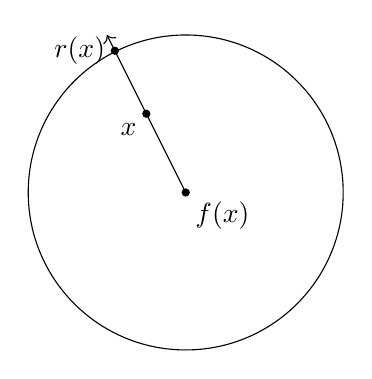
\begin{tikzpicture}
      \draw (0, 0) circle (2);
      \draw[->] (0, 0) to (-1, 2);
      \fill (0, 0) circle (1.5pt) node[below right] {$f(x)$};
      \fill (-0.5, 1) circle (1.5pt) node[below left] {$x$};
      \fill (-0.9, 1.8) circle (1.5pt) node[left] {$r(x)$};
    \end{tikzpicture}
  \end{center}
\end{proof}

\begin{lemma}
    Let \( h: \mathbb{S}^1 \to X \).
    Then \( h \) is nullhomotopic
    if
    \[
      \pi_1(h): \pi_1(\mathbb{S}^1, a) \to \pi_1(X, h(a))
    \]
    is the trivial map.
\end{lemma}

\begin{proof}
    My notes are not easy to read.
    See proof in Hatcher.
\end{proof}

\subsection{Study tips}
Pass (bare minimum):
\begin{enumerate}
  \item topological spaces, cont. maps
    \subitem interior, closure, metric spaces
  \item constructions with topological spaces
    \subitem subspaces
    \subitem products
    \subitem quotients
  \item properties of topological spaces
    \subitem Hausdorff
    \subitem compact
    \subitem connected
  \item which properties are stable under which constructions?
    \subitem find counterexamples, make a table
  \item homotopy theory
    \subitem homotopy
    \subitem path homotopy
    \subitem homotopy equivalence
    \subitem fundamental group
    \subitem \( \pi_1(\mathbb{S}^1) = \mathbb{Z} \)
    \subitem functoriality
\end{enumerate}

Bonus:
\begin{enumerate}
  \item which properties are stable under homotopy equivalence?
\end{enumerate}


\section{Solutions to Exercise sheet 5}
04.04


\end{document}
